% MIT License

% Copyright (c) 2019-2020 Simon Crase

% Permission is hereby granted, free of charge, to any person obtaining a copy
% of this software and associated documentation files (the "Software"), to deal
% in the Software without restriction, including without limitation the rights
% to use, copy, modify, merge, publish, distribute, sublicense, and/or sell
% copies of the Software, and to permit persons to whom the Software is
% furnished to do so, subject to the following conditions:

% The above copyright notice and this permission notice shall be included in all
% copies or substantial portions of the Software.

% THE SOFTWARE IS PROVIDED "AS IS", WITHOUT WARRANTY OF ANY KIND, EXPRESS OR
% IMPLIED, INCLUDING BUT NOT LIMITED TO THE WARRANTIES OF MERCHANTABILITY,
% FITNESS FOR A PARTICULAR PURPOSE AND NONINFRINGEMENT. IN NO EVENT SHALL THE
% AUTHORS OR COPYRIGHT HOLDERS BE LIABLE FOR ANY CLAIM, DAMAGES OR OTHER
% LIABILITY, WHETHER IN AN ACTION OF CONTRACT, TORT OR OTHERWISE, ARISING FROM,
% OUT OF OR IN CONNECTION WITH THE SOFTWARE OR THE USE OR OTHER DEALINGS IN THE
% SOFTWARE.

\documentclass[]{article}
\usepackage{caption,subcaption,graphicx,float,url,amsmath,amssymb,tocloft}
\usepackage[hidelinks]{hyperref}
\usepackage[toc,acronym,nonumberlist]{glossaries}
\usepackage{titling}
\setacronymstyle{long-short}
\usepackage{glossaries-extra}
\graphicspath{{figs/}}
\setlength{\cftsubsecindent}{0em}
\setlength{\cftsecnumwidth}{3em}
\setlength{\cftsubsecnumwidth}{3em} 
% Logo on first page
\pretitle{
	\begin{center}
		
\includegraphics[width=6cm]{KanjiLife}\\	
	}
\posttitle{\end{center}}

%opening
\title{Notes from Origins of Life\\Week4: Early Life}
\author{Simon Crase (compiler)\\simon@greenweaves.nz}

\makeglossaries

\loadglsentries{glossary-entries}

% Prefix section numbers with week number
\renewcommand{\thesection}{4.\arabic{section}}
\renewcommand{\glstextformat}[1]{\textbf{\em #1}}

\begin{document}

\maketitle

\begin{abstract}
   These are my notes from the $4^{th}$ week of the Santa Fe Institute Origins of Life Course\cite{sfi2020}. The course aims to push the field of Origins of Life research forward by bringing new and synthetic thinking to the question of how life emerged from an abiotic world.\\
   The content and images contained herein are the intellectual property of the Santa Fe Institute, with the exception of any errors in transcription, which are my own.
   These notes are distributed in the hope that they will be useful,
   but without any warranty, and without even the implied warranty of
   merchantability or fitness for a particular purpose. All feedback is welcome,
   but I don't necessarily undertake to do anything with it.\\
   \LaTeX source for this week's lectures can be found at\\
   \url{https://github.com/weka511/complexity/tree/master/origins}.
\end{abstract}

\setcounter{tocdepth}{2}
\tableofcontents
\listoffigures
\section[Introduction]{Introduction--Chris Kempes}

We'll discuss evolution in a pre-cellular world, including \glsdisp{gls:autocatalysis}{autocatalytic} networks and molecular evolution, chemical signatures of early life, \glspl{gls:protocell}, and what the \gls{gls:LUCA} might have looked like.

\section[Protocells]{Protocells--Sarah Mauer}

\subsection{Importance of aggregates to origins of life}
We'll look at \glspl{gls:protocell} as a model for the origins of life. \Glspl{gls:protocell} are important for the origins of life because they are aggregates --Figure \ref{fig:ImportanceOfAggregation} \cite{deamer2017role,maurer2011primitive,segre2001lipid}.

\begin{itemize}
	\item  Co-localize and protect metabolic/genetic components
	\item  Define the individual to allow for 	selection
	\item  Direct involvement in metabolism
	\begin{itemize}
		\item 	Chemical gradients
		\item   Electron transfer reactions
		\item   Catalytic (e.g. when a reaction proceeds at a different rate in hydrophobic phase from hydrophilic.)
	\end{itemize}
	\item   Protect metabolic/genetic components
\end{itemize}

\begin{figure}[H]
	\caption{Importance of aggregates to origins of life}\label{fig:ImportanceOfAggregation}
	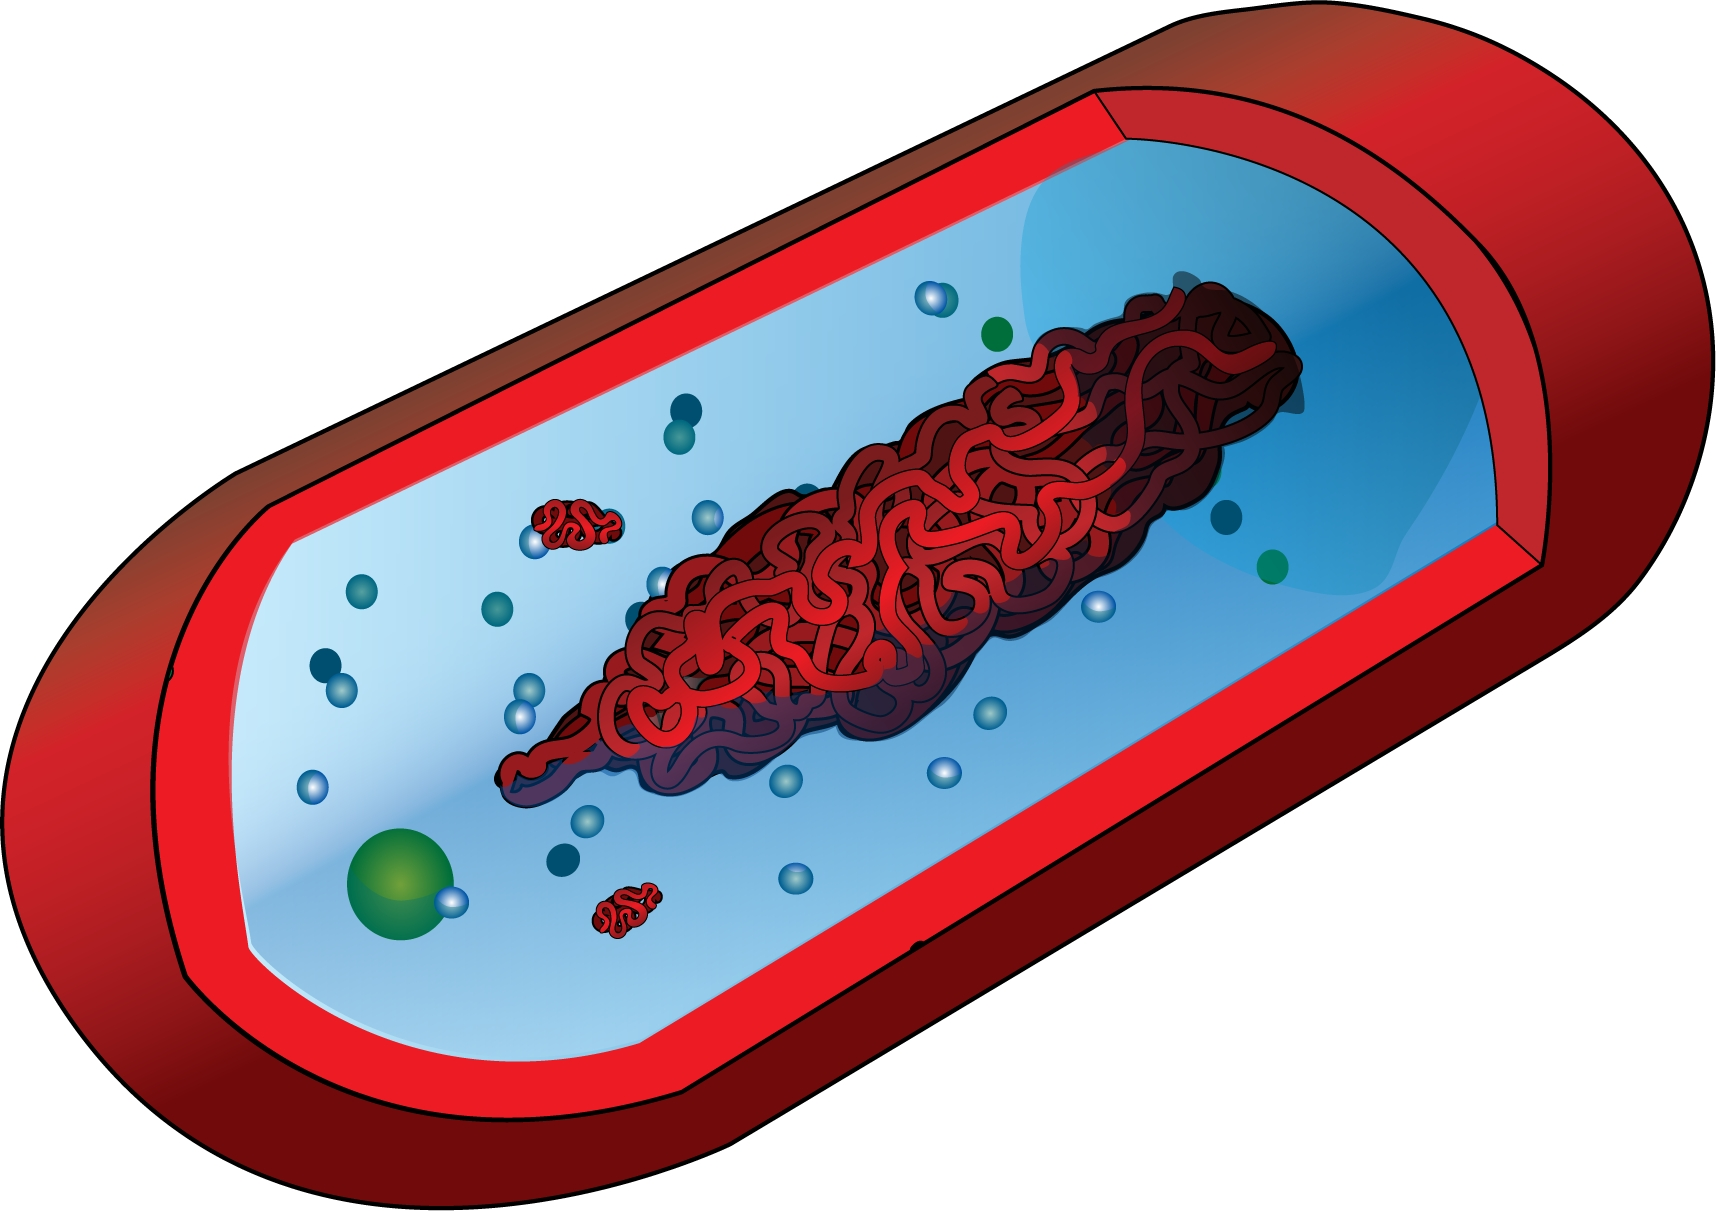
\includegraphics[width=0.9\textwidth]{ImportanceOfAggregation}
\end{figure}

\subsection{Self-assembled structures}

The Aggregates that are used to model the origins of life fall into 3 or maybe 4 categories--Table \ref{table:aggregates}.
Controlled by the hydrophobic effect (entropy) and non-bonding interactions (e.g., hydrogen bonds)

\begin{table}[H]
	\caption{Aggregates that are used to model the origins of life}\label{table:aggregates}
	\begin{tabular}{|l|p{4cm}|p{3cm}|} \hline
		Type & Definition &Biological example\\ \hline
		\Gls{gls:vesicle} (\gls{gls:liposome})& \glsdesc{gls:vesicle}& Cells, membrane bound organelles,\\ \hline
		Oil droplet&
		Nonpolar bulk phase often stabilized by
		amphiphiles&
		Lipoproteins (LDL)\\ \hline
		Coacervate&
		\glsdesc{gls:coacervate}&
		P-bodies, membrane-less organelles\\ \hline
		Inorganic&&Thin films or crystals\\ \hline
	\end{tabular}
\end{table}


\begin{figure}[H]
	\centering
	\caption[Self-assembled structures]{Self-assembled structures\cite{sojo2016origin}}
	\label{fig:self-assembled-structures}
	\begin{subfigure}[b]{0.3\textwidth}
		\centering
		
\includegraphics[width=\textwidth]{SelfAssembled1}
		\caption{Water}
		\label{fig:water}
	\end{subfigure}
	\hfill
	\begin{subfigure}[b]{0.3\textwidth}
		\centering
		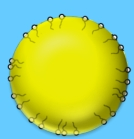
\includegraphics[width=\textwidth]{SelfAssembled2}
		\caption{Not water}
		\label{fig:not-water}
	\end{subfigure}
	\hfill
	\begin{subfigure}[b]{0.3\textwidth}
		\centering
		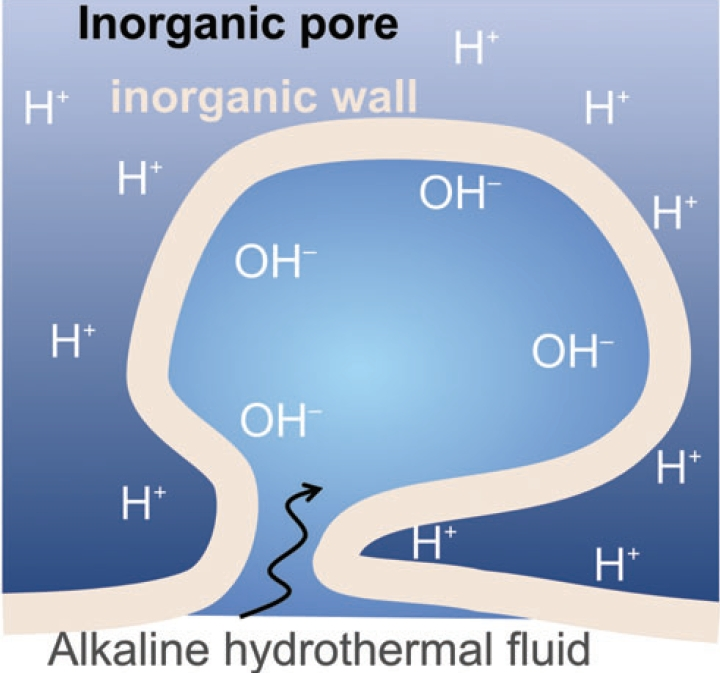
\includegraphics[width=\textwidth]{SelfAssembled3}
		\caption{Proton Gradient across thin inorganic barrier}
		\label{fig:proton-gradient}
	\end{subfigure}

\end{figure}


\subsection{Factors that affect aggregation}
\begin{itemize}
	\item concentration;
	\item temperature;
	\item ionic strength;
	\item pH.
\end{itemize}

\subsection{Protocells and Reactions}

What chemistries do \glspl{gls:protocell} harbour? Figure \ref{fig:ProtocellsAndReactions1} shows several possibilities:
\begin{itemize}
	\item A molecules interact with surface of aggregate through electrostatic interactions or hydrogen bonding;
	\item B hydrophobic effect sequestering non-polar molecule;
	\item C amphiphillic molecule anchored in membrane; 
	\item D molecule sequestered but still in water phase.
\end{itemize}

\begin{figure}[H]
	\caption{Aggregates interacting with molecules that are going to start life}\label{fig:ProtocellsAndReactions1}
	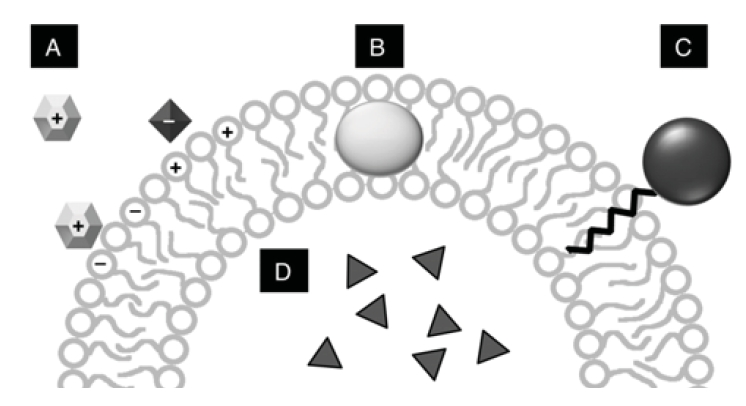
\includegraphics[width=0.9\textwidth]{ProtocellsAndReactions1}
\end{figure}

Figure \ref{fig:ProtocellsAndReactions2} depicts two locations for reactions.
\begin{itemize}
	\item A Surface associated reaction. Substrate becomes Product + Waste, and Waste drifts away. 
	\item B Catalytic network inside membrane, so we need to get rid of Waste.
\end{itemize}
\begin{figure}[H]
	\caption{Two locations for reactions}\label{fig:ProtocellsAndReactions2}
	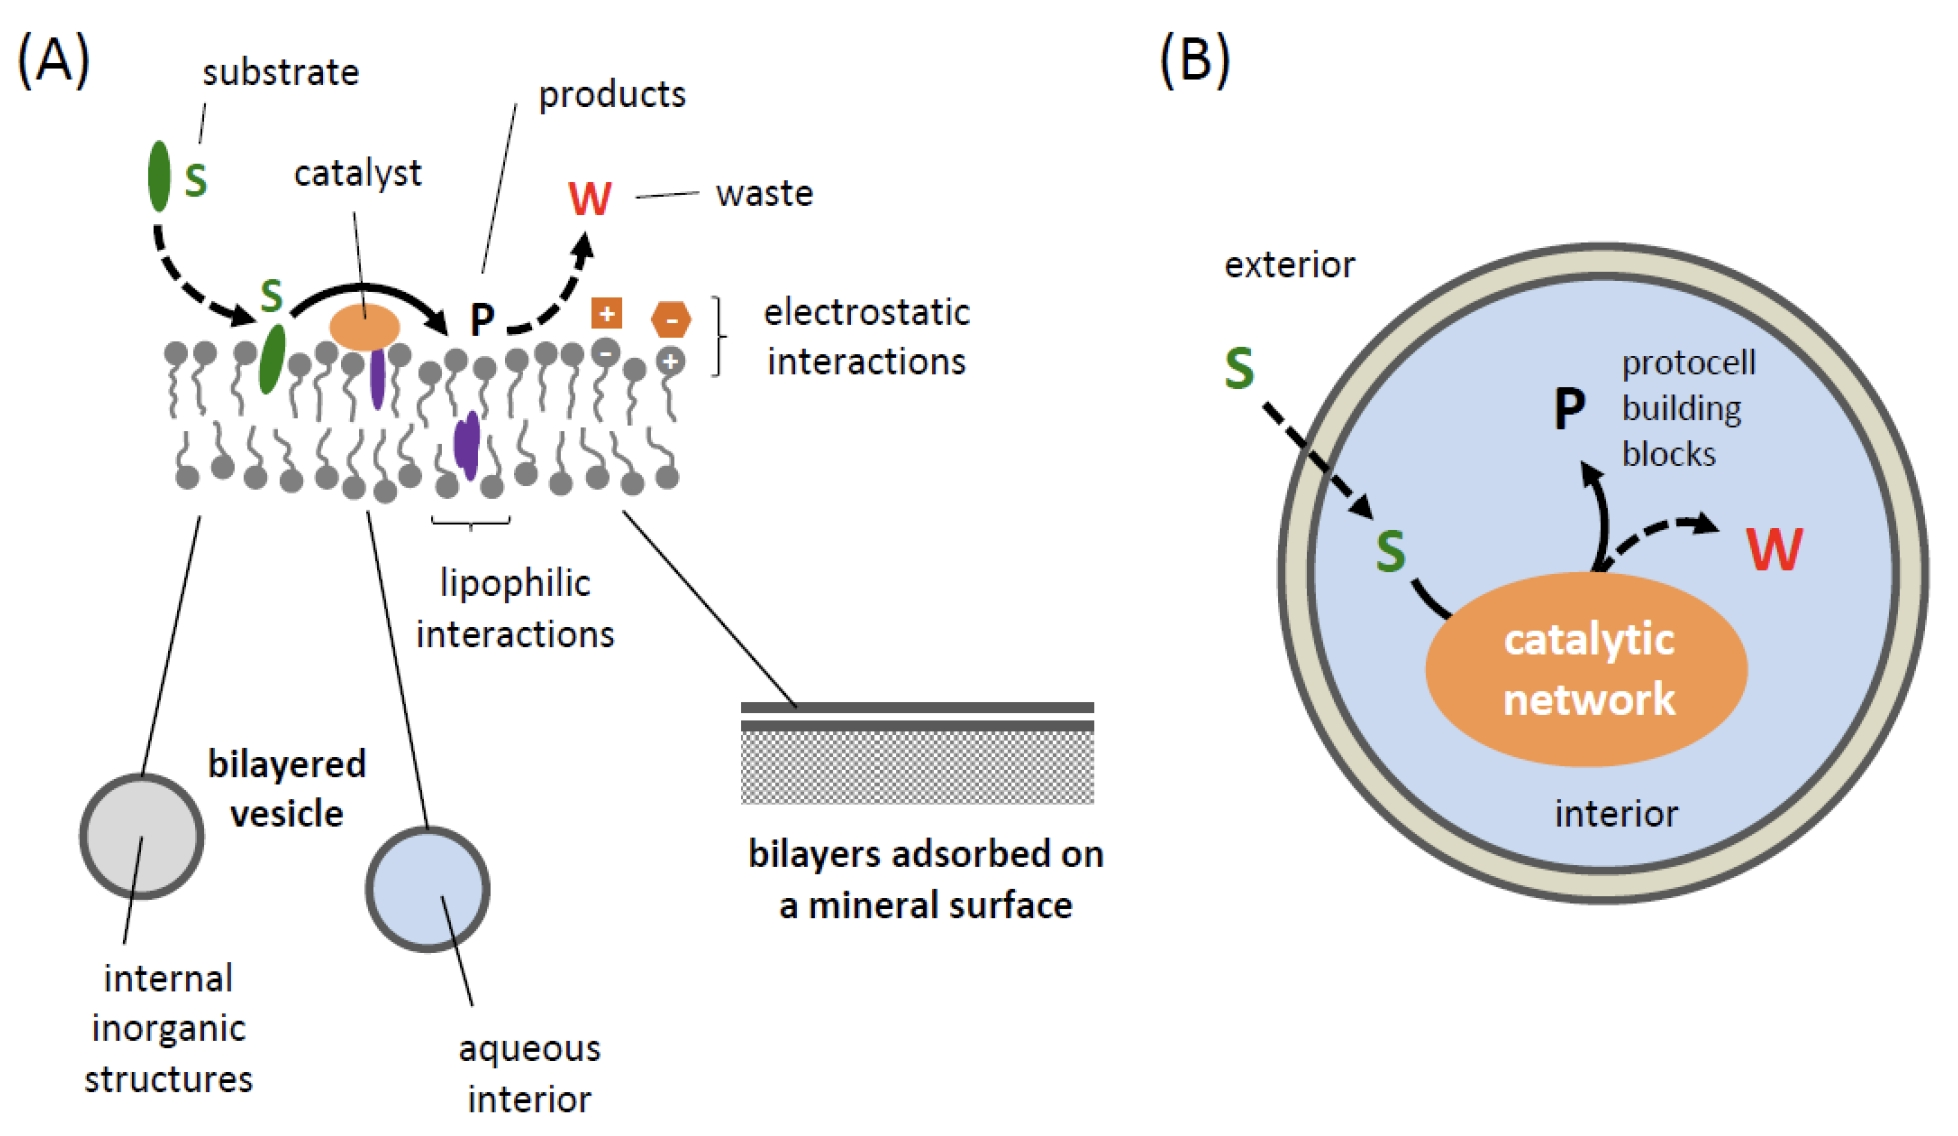
\includegraphics[width=0.9\textwidth]{ProtocellsAndReactions2}
\end{figure}

Figure \ref{fig:ProtocellsAndReactions3} shows an example of a reaction:  the Hammerhead ribosome can self cleave at the red arrow. On the right we see that the reaction is not as fast when it is enclosed in a \gls{gls:vesicle}, because the waste products can't drain away.


\begin{figure}[H]
	\caption{Example of reaction: the Hammerhead ribosome}\label{fig:ProtocellsAndReactions3}
	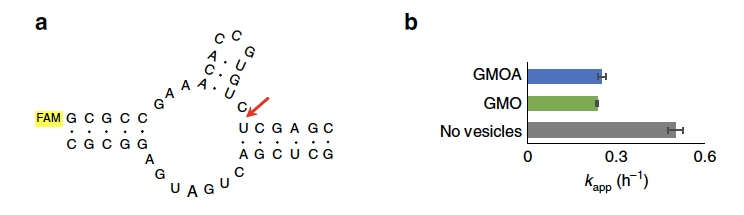
\includegraphics[width=0.9\textwidth]{ProtocellsAndReactions3}
\end{figure}



See \cite{adamala2016programmable,monnard2015current}.

\subsection{Protocell Growth and division}
See movie, where we see growing vesicle stealing material from neighbour. 
Figure \ref{fig:ProtocellGrowthDivision} illustrates \Gls{gls:protocell} growth and division.  

\begin{figure}[H]
	\caption{\Gls{gls:protocell} Growth and division}\label{fig:ProtocellGrowthDivision}
	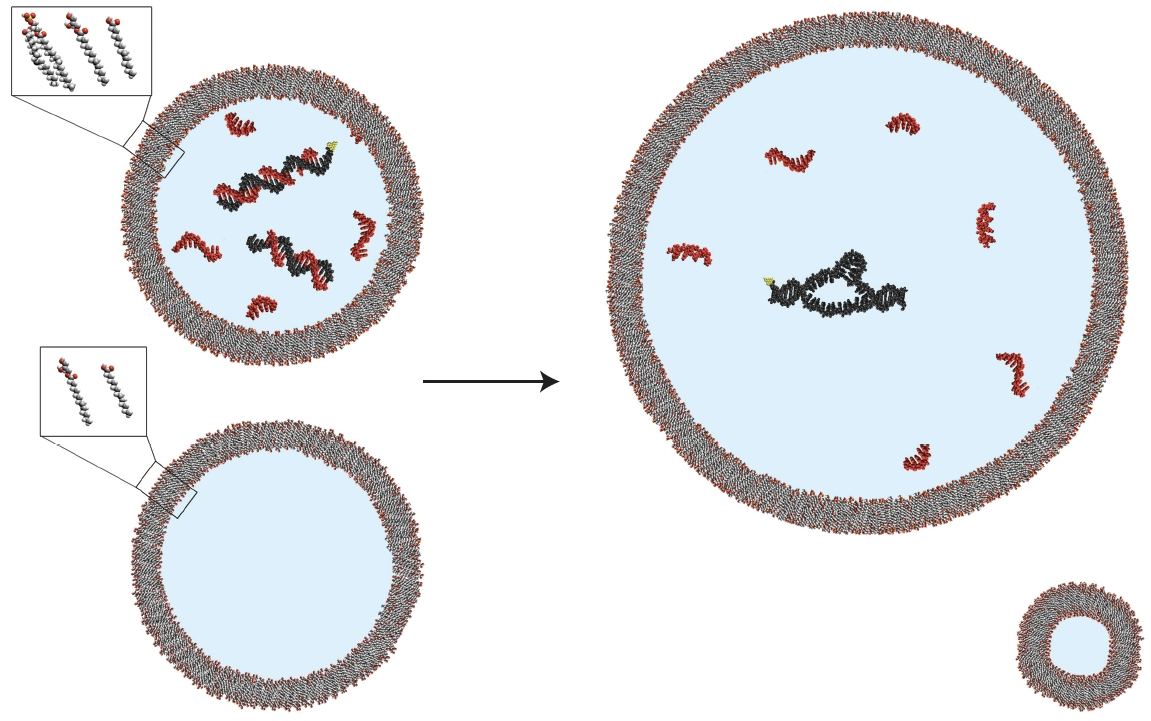
\includegraphics[width=0.9\textwidth]{ProtocellGrowthDivision}
\end{figure}

See  \cite{zhu2012photochemically,chen2004emergence}.

\subsection{Towards LUCA}

In Figure \ref{fig:TowardsLUCA} we see a prebiotic soup, aggregating, decreasing molecular diversity and increasing functional complexity, and moving towards first life. First life can undergo Darwinian evolution towards \gls{gls:LUCA}.
\begin{figure}[H]
	\caption{Towards LUCA}\label{fig:TowardsLUCA}
	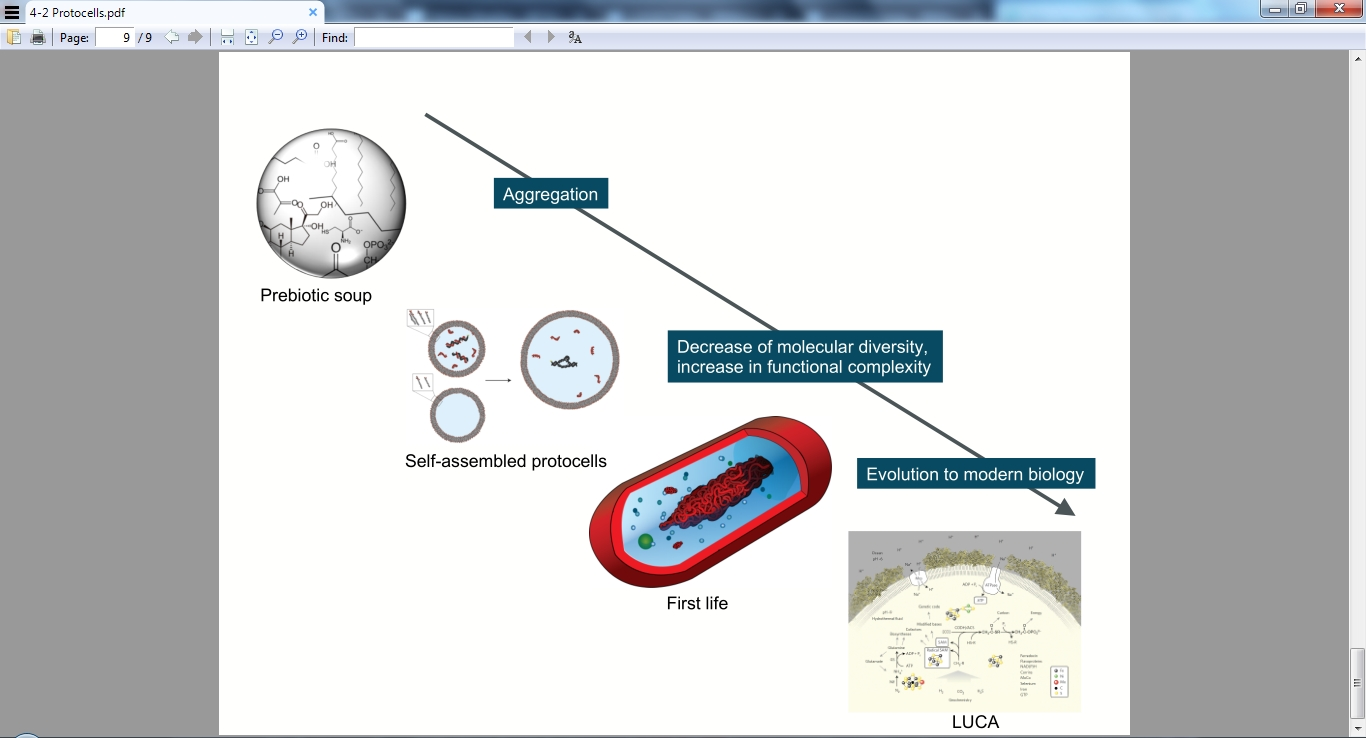
\includegraphics[width=0.9\textwidth]{TowardsLUCA}
\end{figure}

\section[What Did LUCA Look Like?]{What Did \gls{gls:LUCA} Look Like?--Kate Adamala}

Kate discusses the \glsdesc{gls:LUCA} of all Life.

The modern Tree of Life--Figure \ref{fig:TOL4}-- is very diverse in physiology, morphology, and life strategies. But all the diversity  comes from one single ancestor--Figure \ref{fig:TOL_root}.
\begin{figure}[H]
	\caption[The modern Tree of Life]{The modern Tree of Life\cite{hug2016new}}\label{fig:TOL4}
	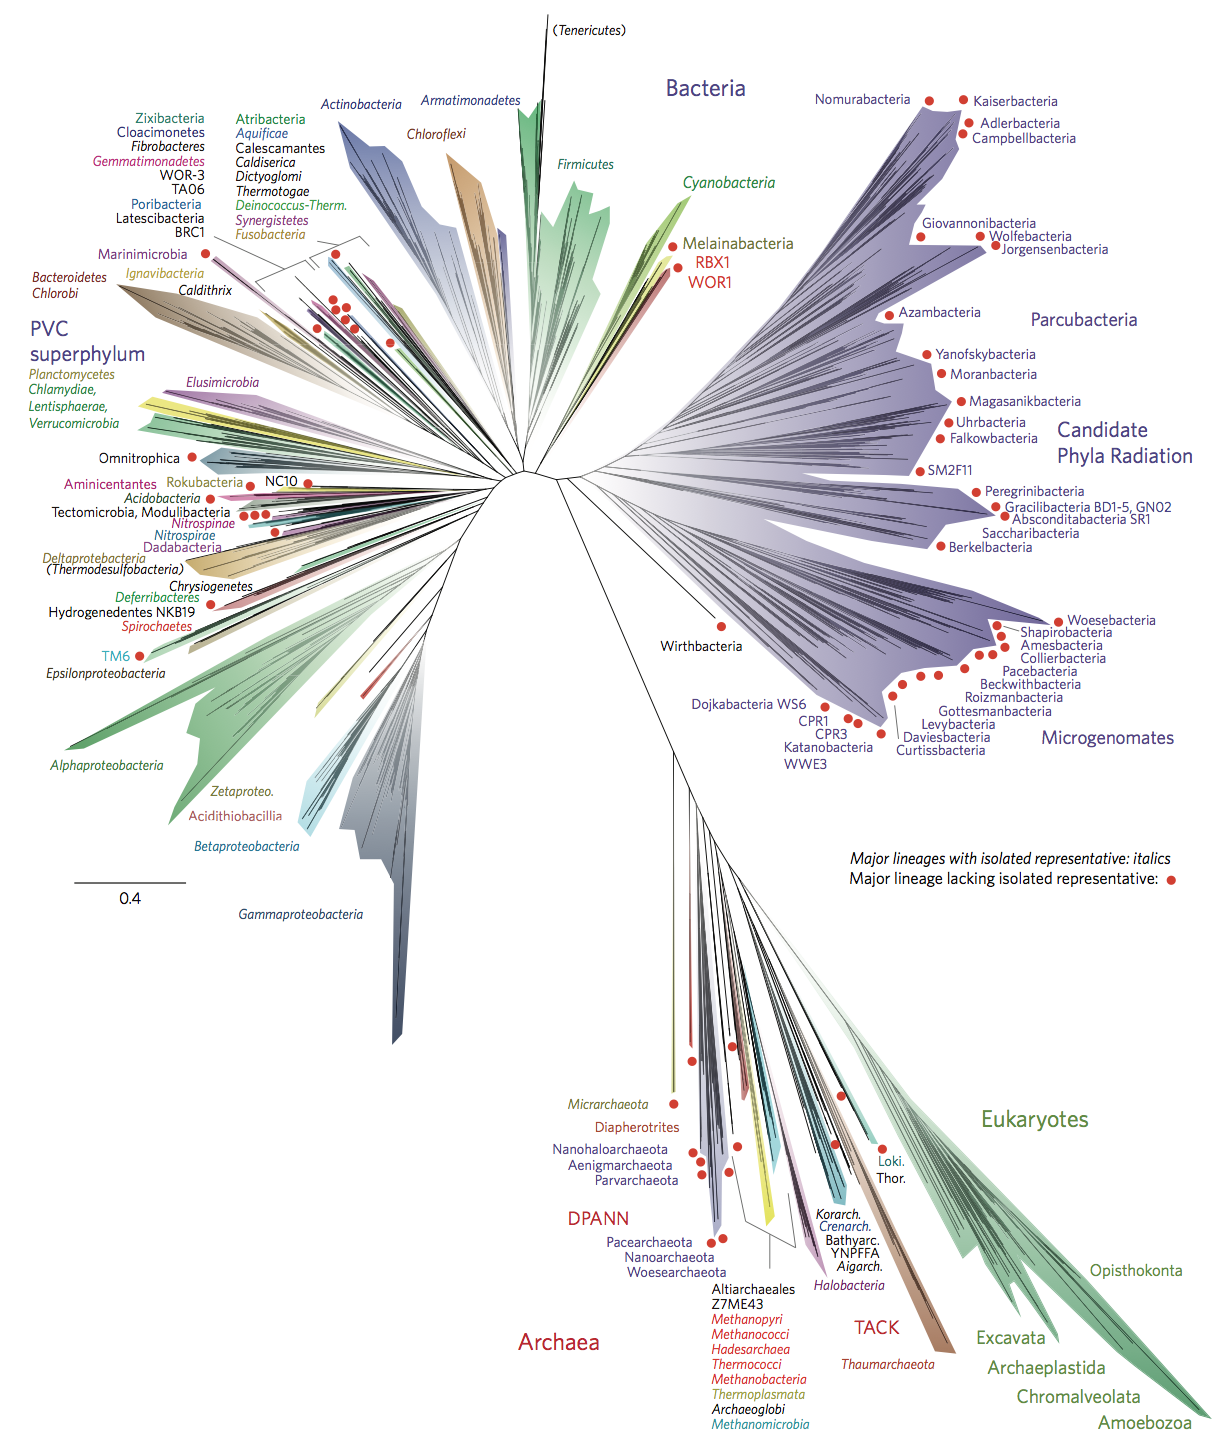
\includegraphics[width=\textwidth]{A_Novel_Representation_Of_The_Tree_Of_Life}
\end{figure}

\begin{figure}[H]
	\caption{All the diversity of Figure \ref{fig:TOL4} comes from one single ancestor.}\label{fig:TOL_root}
	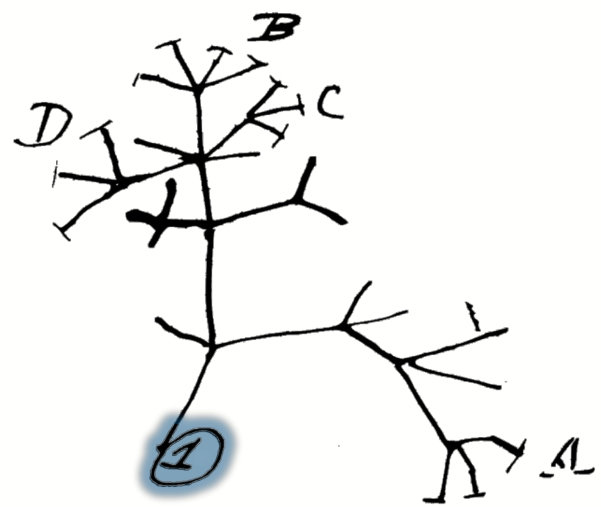
\includegraphics[width=0.9\textwidth]{TOL_root}
\end{figure}

We know that all life came from one population of earliest cells; we know this because, comparing the biochemistry of all known organisms, we can see that all modern life is built on the same principles--Figure \ref{fig:ModernCell}. At one stage, all of life went through the stage of a very simple cell, \gls{gls:LUCA}--Figure \ref{fig:EvolCell}.

\begin{figure}[H]
	\caption{All life came from one population of earliest cells}\label{fig:ModernCell}
	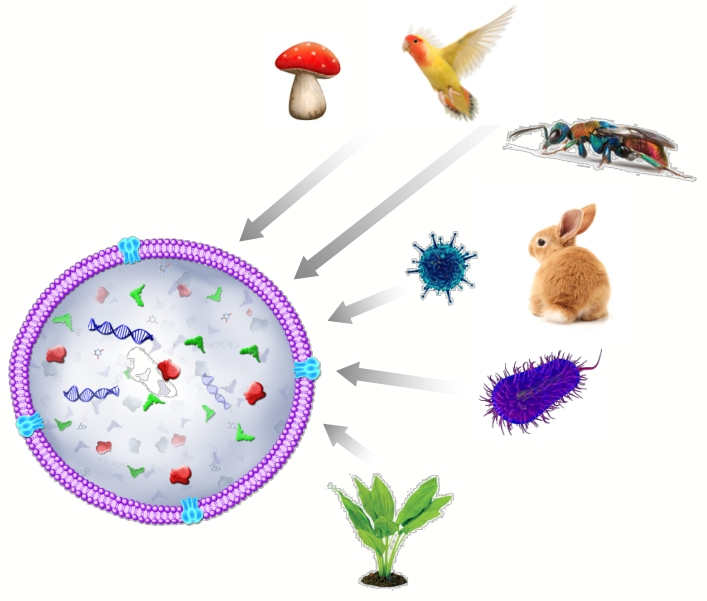
\includegraphics[width=0.9\textwidth]{ModernCell}
\end{figure}

When we consider the way that evolution went, from the simplest building blocks to the complex modern cells, we see that at one point life went through the stage of a very simple cell--Figure \ref{fig:EvolCell}. This was the Last Universal Common Ancestor.
	
\begin{figure}[H]
	\caption{Evolution of Life, showing very simple cell, \gls{gls:LUCA}}\label{fig:EvolCell}
	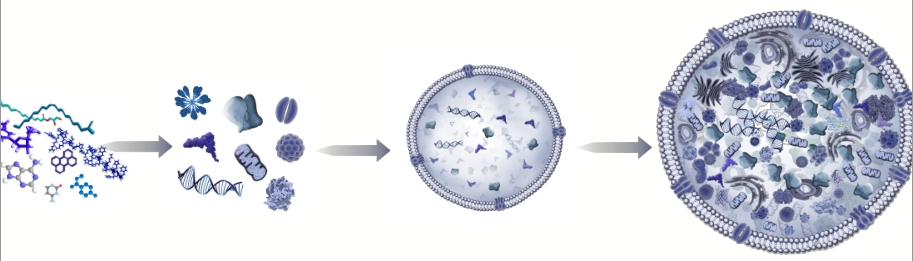
\includegraphics[width=0.9\textwidth]{EvolCell}
\end{figure}

\gls{gls:LUCA} was the ancestor to all modern cells, so it must have possessed the basic mechanisms of  modern cells--Figure \ref{fig:LUCA_Attributes}.

\begin{itemize}
	\item There was a \gls{gls:lipid} bilayer membrane separating the cells from the environment. That membrane was made from lipid derivatives and sterols, just like modern membrane cells.
	\item The membrane was rather impermeable, so there was a need to some transport mechanism for nutrients and waste, most likely protein channels and receptors.
	\item There has to be an energy source to drive whatever is happening inside the membrane. All of modern life uses \gls{gls:ATP} as the energy currency, so it is reasonable to assume that it was used to fuel \gls{gls:LUCA}. Anything made inside the cell--proteins, nucleic acids, cofactors--come from the same set of building blocks, so these had to be present in the ancestor of all domains of life.
	\item To make anything we need protein synthesis, so the translation mechanism must have been present. The core of the modern ribosome was already present, and it hasn't changed much since \gls{gls:LUCA}. In fact the use of \gls{gls:RNA} was the first sign that all life came from a single ancestor. All life uses the same types of \gls{gls:RNA}, suggesting this machinery was already present in \gls{gls:LUCA}.
	\item To make protein we also need \gls{gls:tRNA}.
	\item We need Genes to encode proteins and regulatory elements.
\end{itemize}

\begin{figure}[H]
	\caption{\gls{gls:LUCA} must have possessed the basic mechanisms of  modern cells}\label{fig:LUCA_Attributes}
	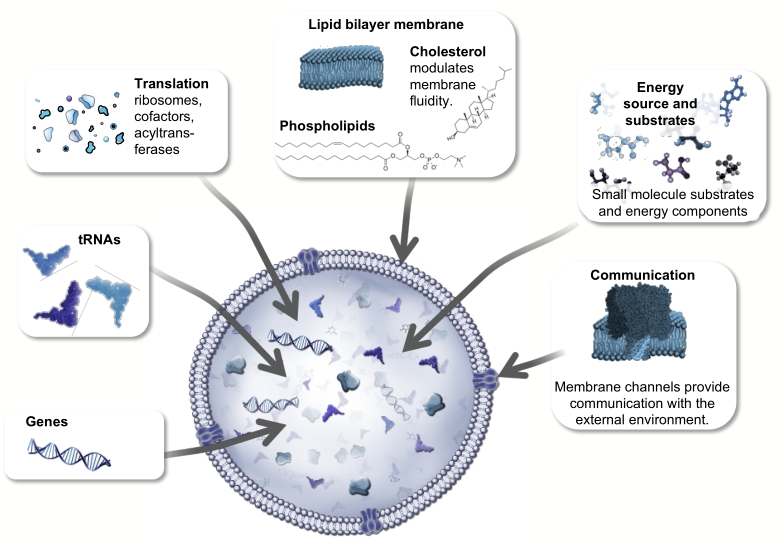
\includegraphics[width=0.9\textwidth]{LUCA_Attributes}
\end{figure}

We know quite a lot about \gls{gls:LUCA}, but much is still unknown. We can deduce much by studying:
\begin{itemize}
	\item biochemical evolution;
	\item the properties of modern cells to see what they share;
	\item geological records to deduce the environment in which \gls{gls:LUCA} lived.
\end{itemize}

References:
\begin{itemize}
	\item \cite{penny1999nature}--cytology of \gls{gls:LUCA};
	\item \cite{weiss2016physiology}--phylogenomic analysis to determine genome of \gls{gls:LUCA};
	\item \cite{torino2013piecing}--reconstruct \gls{gls:LUCA} in the lab.
\end{itemize}

\section[Deducing the environment in which LUCA lived]{Studying geological records to deduce the environment in which \gls{gls:LUCA} lived: Chemical signatures for identifying life in the geological record--Mayuko Nakagawa}

\begin{itemize}
	\item About Biogeochemistry
	\item Fingerprints of life and environment
	\begin{itemize}
		\item Fossils
		\item Mineral compositions
		\item Isotopic signatures
	\end{itemize}
	\item How to use the signatures for identifying lives from 	Earth geological records?
\end{itemize}

\subsection{Biogeochemistry}
Biogeochemistry--The study of:
\begin{itemize}
	\item How chemical elements flow through living systems and their physical environments--Figure \ref{fig:Biogeochemistry}.
	\item Investigate the factors that influence cycles of key 	elements such as bioelements (C, H, N, O, S...).
	
\end{itemize}

\begin{figure}[H]
	\caption[How chemical elements flow through living systems]{How chemical elements flow through living systems\cite{linares-pasten_2018}}\label{fig:Biogeochemistry}
	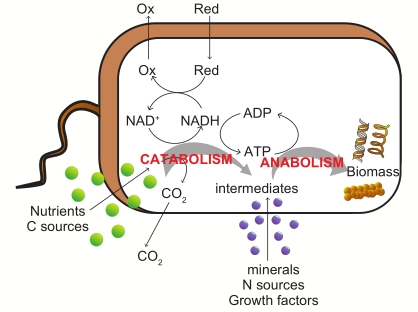
\includegraphics[width=0.9\textwidth]{Biogeochemistry}
\end{figure}

\subsection{Fingerprints of Life}
\begin{itemize}
	\item  DNA information cannot be preserved over geologic time
	scale (thousands ~ million years for eukaryotes' DNA)
	\item Chemical and morphological signatures are utilized
	\begin{itemize}
		\item  Fossils, molecular fossils
		\item Mineral compositions
		\item Isotopic signatures
	\end{itemize}
\end{itemize}

\subsubsection{Isotopic signatures}: Isotope variants of a particular chemical element
which differ in neutron number--Figure \ref{fig:CarbonIsotopes}.
\begin{itemize}
	\item  Stable isotope
	\begin{itemize}
		\item do not decay into other elements.
		\item Behaviour is slightly different by the mass, useful for understanding 	material cycle--Figure \ref{fig:IsotopicEffects}.
	\end{itemize}
	\item Radioactive isotope: one having an unstable nucleus and which emits characteristic radiation during its decay to a stable form- e.g. $^3H$, $^14C$
\end{itemize}

\begin{figure}[H]
	\caption{Carbon Isotopes}\label{fig:CarbonIsotopes}
	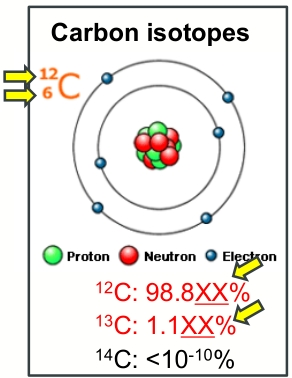
\includegraphics[width=0.9\textwidth]{CarbonIsotopes}
\end{figure}


\begin{itemize}
	\item \textit{Kinetic isotopic effect}:
	Isotope ratio is changed by kinetic reactions 	(e.g.) the isotopic ratios are changed between substrates and products reflecting the metabolic processes--Figure \ref{fig:KineticIsotopicEffects}. \begin{align*}
	^{12}CO_2 + H_2O \rightarrow&^{12}CH_2O + O_2 \text{, runs slightly faster than}\\
	^{13}CO_2 + H_2O \rightarrow&^{13}CH_2O + O_2 
	\end{align*}
	\item \textit{Equilibrium isotopic effect}:
	Isotope ratio is changed by equilibrium reactions.
	e.g.) Temperature effect, phase (gas, liquid, solid)
	$^{18}O$ ( $^{16}O$) is more (less) enriched in liquid than gas phase--Figure \ref{fig:EquilibriumIsotopicEffects}
\end{itemize}

\begin{figure}[H]
	\caption{Isotopic Effects}\label{fig:IsotopicEffects}
	\begin{subfigure}[t]{0.45\textwidth}
		\caption{Kinetic Isotopic Effect}\label{fig:KineticIsotopicEffects}
		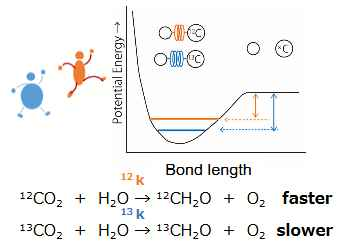
\includegraphics[width=\textwidth]{KineticIsotope1}
	\end{subfigure}
	\begin{subfigure}[t]{0.45\textwidth}
		\caption{Equilibrium Isotopic Effect}\label{fig:EquilibriumIsotopicEffects}
		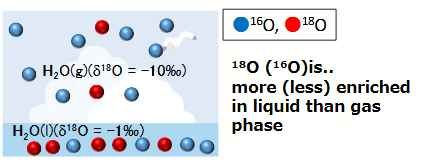
\includegraphics[width=\textwidth]{EquilibriumIsotopicEffect}
	\end{subfigure}
\end{figure}

These isotopic effects provide a characteristic range of values on target compounds. Using these characteristics we can understand the sources and consumption for target compounds. In a natural environment environmental conditions interact with the players in the ecosystem. The isotopic signatures are investigated with a modern environment with varying conditions. The datasets investigated with a modern environment are utilized for decoding the geological record.
\begin{figure}[H]
	\caption{Isotopic Signatures}
	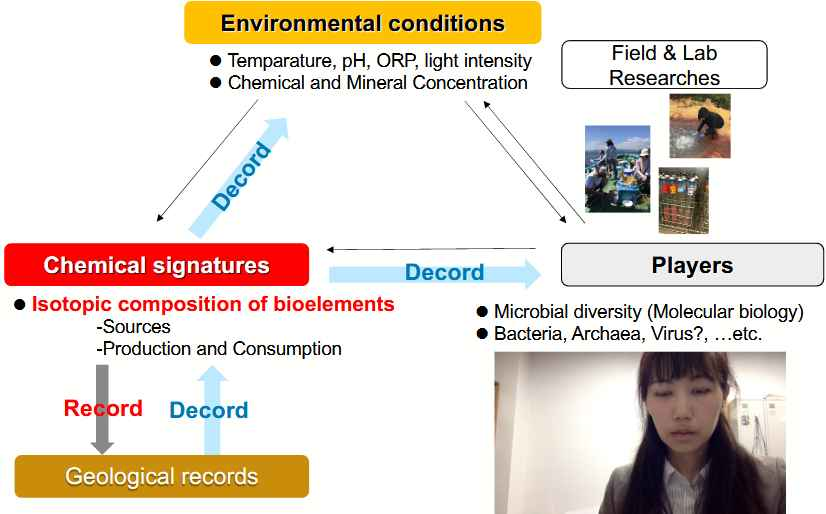
\includegraphics[width=0.8\textwidth]{IsotopicSignatures}
\end{figure}

\begin{figure}[H]
	\caption{Earth environment interacts with origin and evolution of life}\label{fig:Timeline}
	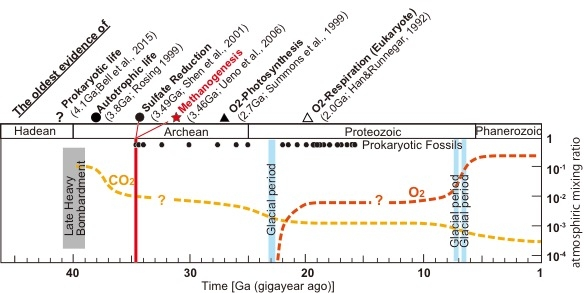
\includegraphics[width=0.9\textwidth]{Timeline}
\end{figure}

\begin{itemize}
	\item O2 level is important for evolution of life:
	\begin{itemize}
		\item the content of oxidized minerals and S isotope ratios are used for
		signatures of O2 level
	\end{itemize}
	\item  Small C isotope ratio ($\delta^{13}C$) of microfossils
	\begin{itemize}
		\item 	The difference of $\delta^{13}C$ values between carbonate and organic carbon ($<13\%$) indicated the possibility of Acetyl-CoA pathway
		and/or Calvin cycle product.
	\end{itemize}
\end{itemize}

Isotopic signature for Methanogens:
\begin{itemize}
	\item The sample rocks ($\approx 3.5Ga$); at the Dresser Formation at the North Pole area in Pilbara craton, Western Australia \cite{ueno2006evidence},
	\item Fluid inclusion; Tiny bubble of liquid or gas trapped inside a solid mineral-phase--Figure \ref{fig:FluidInclusionInTheRock}
	\item Measure C isotope ratio ( $\delta^{13}C$) of $CO_2$ and $CH_4$ in fluid inclusion
\end{itemize}

\begin{figure}[H]
	\caption{Fluid inclusion in the rock}\label{fig:FluidInclusionInTheRock}
	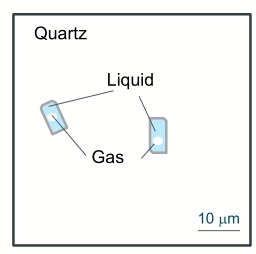
\includegraphics[width=0.9\textwidth]{FluidInclusionInTheRock}
\end{figure}

Isotopic signature for Methanogens. Figure \ref{fig:ueno_comparison} supports the idea that the methane is biogenic.
\begin{itemize}
	\item Methane production processes (Biogenic)
	\begin{itemize}
		\item 	Acetate Fermentation
		\item $CO_2$ reduction
	\end{itemize}
	\item Methane production processes (Abiotic)
	\begin{itemize}
		\item Thermogenic decomposition,
		\item Fischer-Tropsch reaction
	\end{itemize}
\end{itemize}

\begin{figure}[H]
	\caption{Comparison with present-day hydrothermal system}\label{fig:ueno_comparison}
	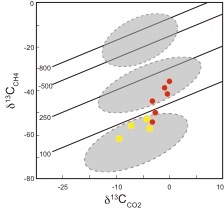
\includegraphics[width=0.9\textwidth]{ueno_comparison}
\end{figure}

Take Home Message: Signatures of life:
\begin{itemize}
	\item Chemical signatures, especially stable isotope information, are important tool for identifying the biogenic signatures preserved in geological records
	\item To understand how to record and decode the signatures, researches on modern earth material cycle and organisms are 	necessary.
\end{itemize}

Suggested Reading:

\cite{sharp2017principles,allegre2008isotope}

References:
\cite{ueno2006evidence,bell2015potentially,rosing199913c,shen2001isotopic,summons19992,han1992megascopic}

\section{RNA}

\subsection[The RNA World]{The RNA World--Tony Z. Jia}

\subsubsection{The Modern Cell}

All living organisms are made up of cells, and each cell is composed of a boundary, made up of a phospholipid bilayer--Figure \ref{fig:PhosphoLipidBilayer}.\begin{itemize}
	\item  Within this bilayer is a genetic molecule, DNA, which undergoes self-replication, so that copies of itself can be transmitted to daughter cells during self replication. This process is catalyzed by protein enzymes--Figure \ref{fig:DNA_self_rep}.
	\item DNA can also be transcribed to a messenger molecule--Figure  \ref{fig:DNA_transcription}.
	\item The RNA is translated to proteins, catalyzed by the ribosome--Figure \ref{fig:ModernCellSchematic}.
\end{itemize}
These process give rise to the Central Dogma--Figure \ref{fig:CentralDogmaModernCell}.
\begin{figure}[H]
	\caption[The Modern Cell gives rise to the Central Dogma]{The Modern Cell gives rise to the Central Dogma: this process of going from DNA to RNA to proteins is exhibited in all forms of modern life.}
	\begin{subfigure}[m]{0.45\textwidth}
		\caption{Each cell is composed of a boundary, made up of a phospholipid bilayer.}\label{fig:PhosphoLipidBilayer}
		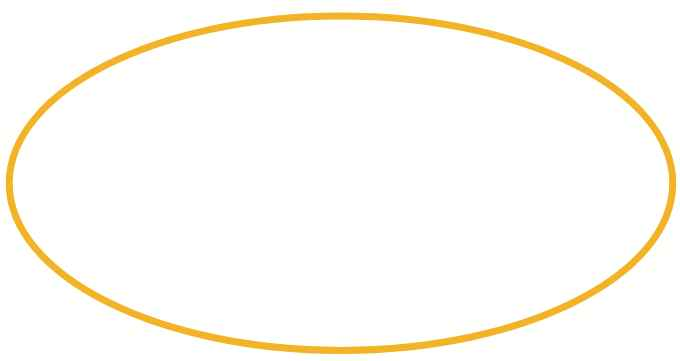
\includegraphics[width=\textwidth]{PhosphoLipidBilayer}
	\end{subfigure}
	\begin{subfigure}[m]{0.45\textwidth}
		\caption{ Within this bilayer is a genetic molecule, DNA, which undergoes self-replication, so that copies of itself can be transmitted to daughter cells during self replication.}\label{fig:DNA_self_rep}
		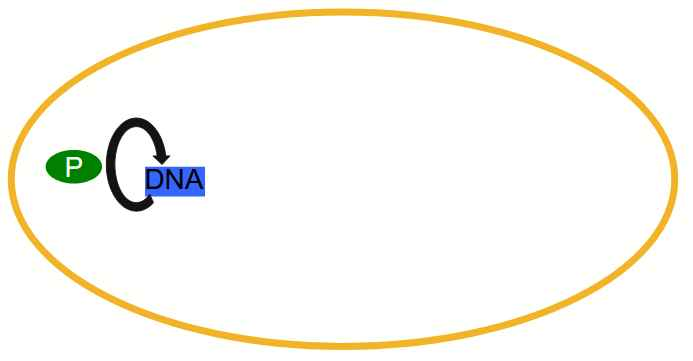
\includegraphics[width=\textwidth]{DNA_self_rep}
	\end{subfigure}
	\begin{subfigure}[m]{0.45\textwidth}
		\caption{DNA can also be transcribed to a messenger molecule.}\label{fig:DNA_transcription}
		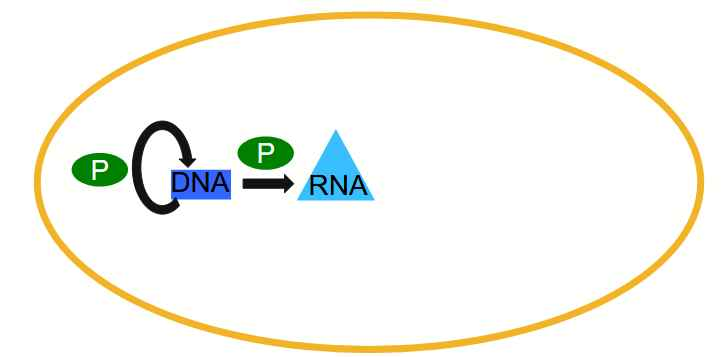
\includegraphics[width=\textwidth]{DNA_transcription}
	\end{subfigure}
	\begin{subfigure}[m]{0.45\textwidth}
		\caption{The RNA is translated to proteins, catalyzed by the ribosome.}\label{fig:ModernCellSchematic}
		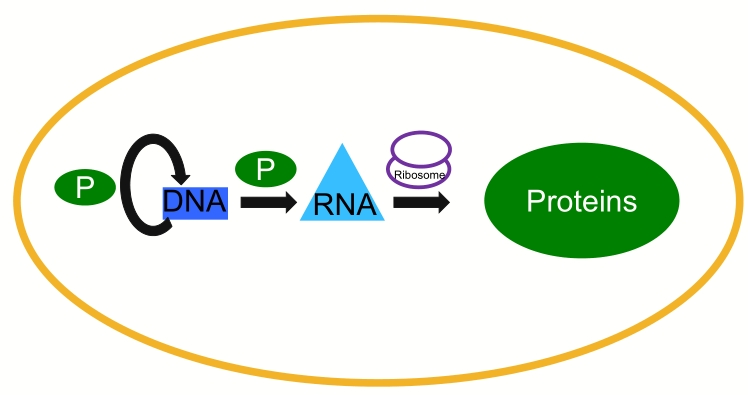
\includegraphics[width=\textwidth]{ModernCellSchematic}
	\end{subfigure}
	\begin{center}
		\begin{subfigure}[m]{0.7\textwidth}
		\caption{This process is known as the Central Dogma}\label{fig:CentralDogmaModernCell}
		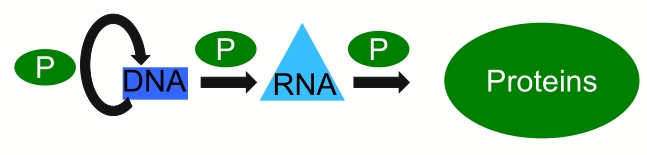
\includegraphics[width=\textwidth]{CentralDogmaModernCell}
	\end{subfigure}
	\end{center}
\end{figure}

\subsubsection{RNA World Theory}
\gls{gls:RNA} can perform the same functions as DNA and proteins:
\begin{itemize}
	\item   it can store and pass down genetic information--Figure \ref{fig:RNA_WorldTheory}
	\item it  can catalyze chemical processes (ribozymes)--Figure \ref{fig:RNA_can_catalyze_chemical_processes}\cite{scott2013hammerhead}
\end{itemize}
\begin{figure}[H]
	\caption[RNA can store and pass down genetic information similar to DNA]{\gls{gls:RNA}  can store and pass down genetic information similar to \gls{gls:DNA} }\label{fig:RNA_WorldTheory}
	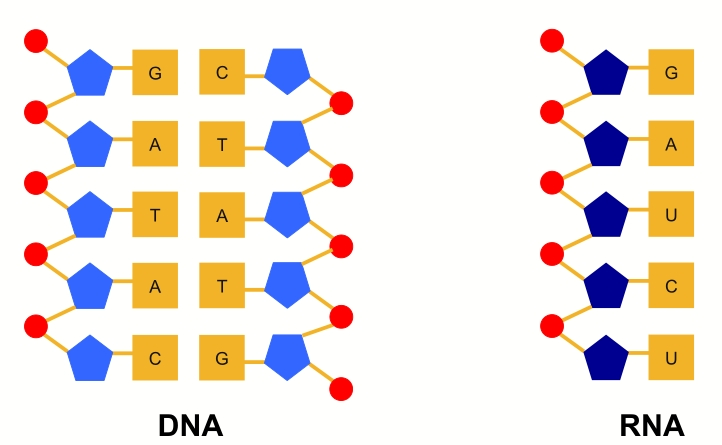
\includegraphics[width=0.9\textwidth]{RNA_WorldTheory}
\end{figure}

\begin{figure}[H]
	\caption{RNA can catalyze chemical processes}\label{fig:RNA_can_catalyze_chemical_processes}
	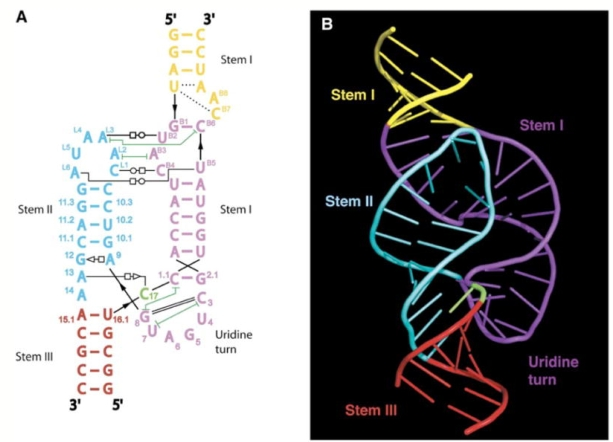
\includegraphics[width=0.9\textwidth]{RNA_can_catalyze_chemical_processes}
\end{figure}

We'll consider an early living system--Figure \ref{fig:RNA_WorldTheory1}, where the genetic material is RNA:
\begin{itemize}
	\item need RNA to be able to replicate and evolve;
	\item then system can grow, replicate, and divide.
\end{itemize}
 

\begin{figure}[H]
	\caption[An early living system, where the genetic material is RNA.]{An early living system, where the genetic material is RNA\cite{blain2014progress}.}\label{fig:RNA_WorldTheory1}
	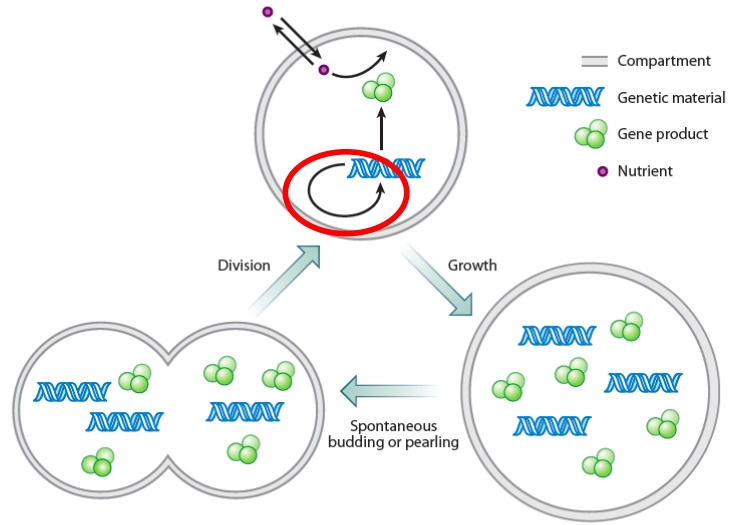
\includegraphics[width=0.9\textwidth]{RNA_WorldTheory1}
\end{figure}

There are many ways the self-replication of RNA has been postulated to occur. At some point in evolution, it is very likely that an RNA ribozyme, i.e. a catalytic RNA that could catalyze replication and polymerization of other RNA molecules, would have been necessary for such a system to have been maintained. But what would have happened \emph{before} the emergence of such an RNA ribozyme? Figure \ref{fig:NonenzymaticRNA_Polymerization} shows one possibility:

\begin{itemize}
	\item monomers bind to RNA, based on complements (chemistry, not biology!)--Figure \ref{fig:MonomerBinding};
	\item monomers are then polymerized, so we get complementary strand--Figure \ref{fig:RNA_polymerization_somehow};
	\begin{itemize}
		\item one mechanism involves the Leaving Group\footnote{All Leaving Groups discussed here are laboratory analogs. They aren't necessarily what was used, but they enable us to study processes in the lab.} in the Template, a slightly activated group that catalyzes extension--Figure \ref{fig:RNA_polymerization_somehow1};
		\item Leaving Group may be 2-Methylimidazole
	\end{itemize} 
	\item at this point, RNA strand has replicated itself--Figure \ref{fig:self:rep:complete}.
\end{itemize}

\begin{figure}[H]
	\caption[Nonenzymatic RNA Polymerization]{Nonenzymatic RNA Polymerization\cite{blain2014progress}}\label{fig:NonenzymaticRNA_Polymerization}
	\begin{subfigure}[m]{0.45\textwidth}
		\caption{monomers bind to RNA, based on complements}\label{fig:MonomerBinding}
		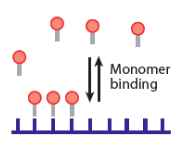
\includegraphics[width=\textwidth]{MonomerBinding}
	\end{subfigure}
	\begin{subfigure}[m]{0.45\textwidth}
		\caption{Monomers are then polymerized, so we get complementary strand}\label{fig:RNA_polymerization_somehow}
		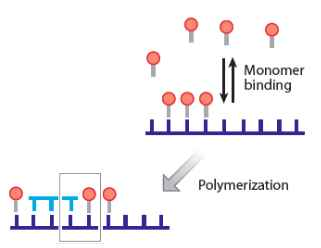
\includegraphics[width=\textwidth]{RNA_polymerization_somehow}
	\end{subfigure}
	\begin{subfigure}[b]{0.45\textwidth}
		\caption{Activated monomers: a monomer is slightly activated by a \gls{gls:leaving group}, which catalyzes the extension of the complementary RNA strand so it can incorporate new monomers.}\label{fig:RNA_polymerization_somehow1}
		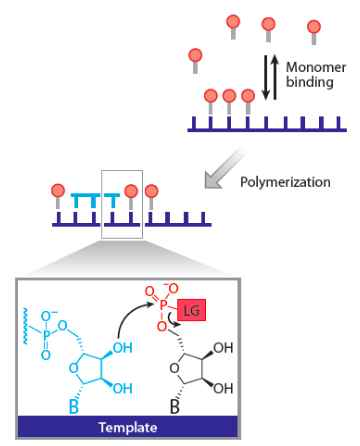
\includegraphics[width=\textwidth]{RNA_polymerization_somehow1}
	\end{subfigure}
	\begin{subfigure}[b]{0.45\textwidth}
		\caption{Complementary Strand has been formed--RNA has successfully replicated itself. The leaving group has often be postulated to occur through 2-Methylimidazole(pictured).}\label{fig:self:rep:complete}
		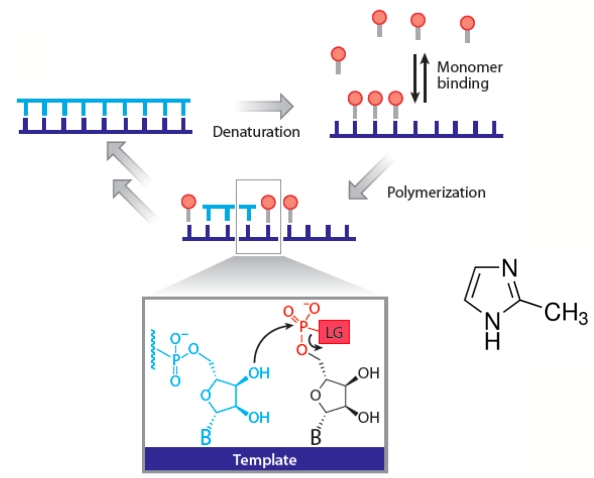
\includegraphics[width=\textwidth]{NonenzymaticRNA_Polymerization}
	\end{subfigure}
\end{figure}


There are still some outstanding issues:
\begin{itemize}
	\item How does denaturation step happen in Figure \ref{fig:NonenzymaticRNA_Polymerization}? Otherwise we'd use up all RNA, and there would be no evolution. Figure \ref{fig:PrebioticRNA_StrandSeparation} shows one possibility--pH cycling.
	\item Polymerization isn't as fast as we'd like, and there is some degrading. Figure \ref{fig:ChangeLeavingGroup} shows one possibility: replace 2-Methylimidazole with 2-aminoimidazole\cite{li2017enhanced}, which gives a much faster reaction.
	\item  RNA is very labile to hydrolysis, and it \textit{degrades quickly}, especially if solutions aren't clean. Need Magnesium cations for polymerization, but this also causes degradation. Maybe use a different cation, such as Iron--Figure \ref{fig:RNA_polymerization_via_iron}\cite{blain2014progress}, but this works only if there is no oxygen to convert $Fe^{2+}$ to $Fe^{3+}$.
\end{itemize}

\begin{figure}[H]
	\caption{Prebiotic RNA strand separation}\label{fig:PrebioticRNA_StrandSeparation}
	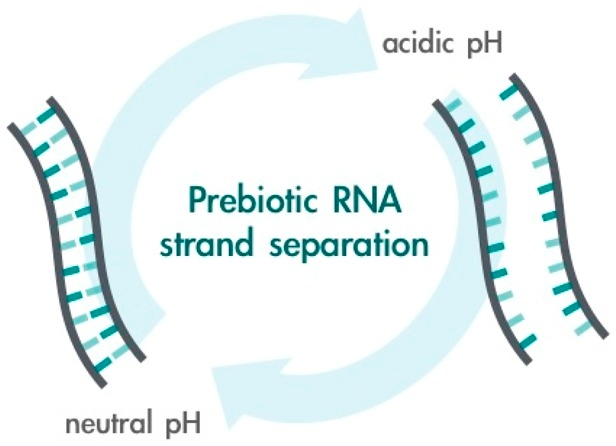
\includegraphics[width=0.9\textwidth]{PrebioticRNA_StrandSeparation}
\end{figure}

\begin{figure}[H]
	\caption{Replace 2-Methylimidazole with 2-aminoimidazole}\label{fig:ChangeLeavingGroup}
	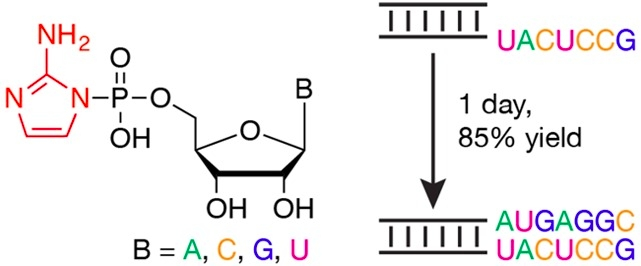
\includegraphics[width=0.9\textwidth]{ChangeLeavingGroup}
\end{figure}

\begin{figure}[H]
	\caption{Use Reduced Iron in an oxygen free chamber.}\label{fig:RNA_polymerization_via_iron}
	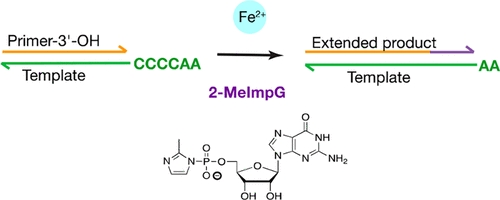
\includegraphics[width=0.9\textwidth]{RNA_polymerization_via_iron}
\end{figure}

See \cite{robertson2012origins,joyce2018protocells} for details of the origins of the RNA world, and its processes, and \cite{hud2018searching} for information on the hypothetical pre-RNA world. Finally, it is possible to have living systems with more than 4 bases  \cite{hoshika2019hachimoji}.

\subsection[Molecular Evolution in the Lab]{Molecular Evolution in the Lab--Mark A. Ditzler}

A method called ''In vitro evolution'' allows us to observe the evolution of molecules in a test tube--Figure \ref{fig:InVitroEvolution_Darwin}. It has been used to study several classes of molecules:
\begin{itemize}
	\item Proteins
	\item Ribonucleic acids (RNAs)
	\item Non-biological RNA-like molecules (like RNA, but with different backbone or different base-pairs)
\end{itemize}

\begin{figure}[H]
	\begin{center}
		\caption[In vitro evolution]{In vitro evolution allows us to observe the evolution of molecules in a test tube}\label{fig:InVitroEvolution_Darwin}
		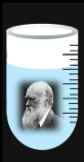
\includegraphics[width=0.6\textwidth]{InVitroEvolution_Darwin}
	\end{center}
\end{figure}

In vitro evolution allows us to answer two broad questions:
\begin{itemize}
	\item what \textit{can} these molecules do?
	\item how \textit{can} they evolve?
\end{itemize}
This study is independent of biology and specific evolutionary histories.

How does In vitro evolution work--Figure \ref{fig:InVitroEvolution}?

\begin{itemize}
	\item Start with a diverse population, e.g. $\approx 10^{15}$ 
	unique sequences of protein, RNA, or RNA-like molecules
	\item Select: isolate molecules that have the desired function
	\begin{itemize}
		\item Carry out chemical reactions: Ligation, transfer of functional groups,
		oxidation/reduction, isomerization, etc
		\item Bind other biomolecules: 	Wide variety of metabolites and proteins
	\end{itemize}
	\item Use enzymatic steps to make many copies of isolated molecules
	\item There will be some mutations (mistakes), so we get additional diversity
	\item Repeated selection will produce more copies of ''better'' sequences
	\item Repeat until we end up with ''really good'' sequences--Figure \ref{fig:InVitroEvolutionRepeat}
\end{itemize}

\begin{figure}[H]
	\caption[How does In vitro evolution work? First steps.]{How does In vitro evolution work? First steps: start with a very diverse collection of molecules}\label{fig:InVitroEvolution}
	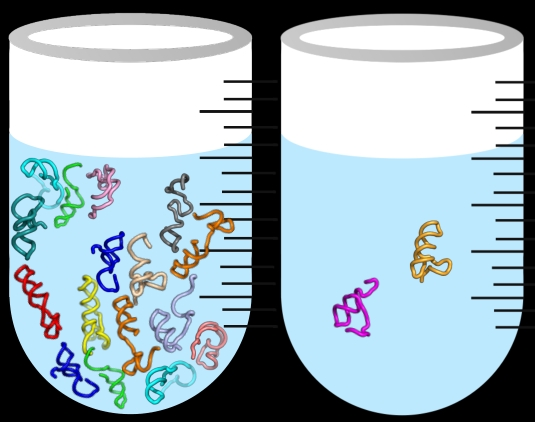
\includegraphics[width=0.9\textwidth]{InVitroEvolution}
\end{figure}

\begin{figure}[H]
	\caption{How does In vitro evolution work? Overview}\label{fig:InVitroEvolutionRepeat}
	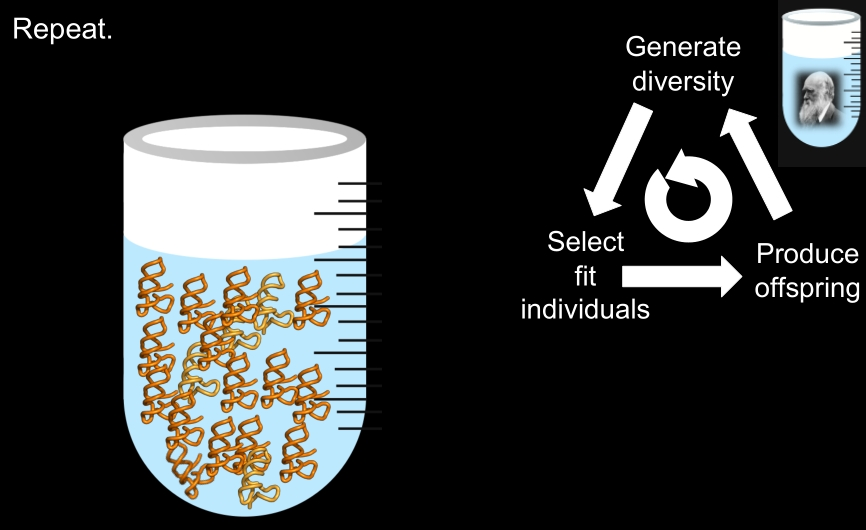
\includegraphics[width=0.9\textwidth]{InVitroEvolutionRepeat}
\end{figure}

What have we learned?
\begin{itemize}
	\item what \textit{can} these molecules do?
	\begin{itemize}
		\item Very simple proteins can carry out chemical reactions\cite{seelig2007selection}
		\item RNA can catalyze many classes of chemical reactions\cite{chen2007ribozyme}
		\item RNA can bind a wide range of biomolecules\cite{gold2012aptamers}
		\item RNA-like molecules can do many of the same functions as RNA\cite{sefah2014vitro,pinheiro2012synthetic}
	\end{itemize}
	\item how \textit{can} they evolve?
		\begin{itemize}
		\item Proteins evolved in vitro look different from proteins in modern biology\cite{mansy2007structure}
		\item Highly active molecules with complex functions are extremely rare among random sequences \cite{bartel1993isolation}
		\item Neutral point-mutations may plan a smaller role in evolution of new structure and functions than we previously thought\cite{petrie2014limits,pressman2019mapping}
	\end{itemize}
\end{itemize}

Suggested Reading
\begin{itemize}
	\item \cite{joyce2007forty}--an excellent review of the history of in vitro evolution as told by one of its most accomplished practitioners.
	\item \cite{seelig2007selection}--an excellent example of the in vitro evolution of a protein
	\item \cite{chen2007ribozyme}--a very well-written patent filed in 1991 by one of the pioneers of in-vitro evolution for a specific form of in vitro evolution known as SELEX.
\end{itemize}


\section{Autocatalysis}

\subsection[Autocatalytic Sets: A Cooperative Origin of Life--Wim Hordijk
]{Autocatalytic Sets: A Cooperative Origin of Life--Wim Hordijk}

The dominant paradigm in the origins of life is the RNA World. RNA molecules fall into a complicated 3 dimensional structure--Figure \ref{fig:RNA}. This allows them to be able to be chemically active; in particular it allows them to catalyze reactions of other RNA molecules.

\begin{figure}[H]
	\caption[RNA molecules fall into a complicated 3 dimensional structure]{RNA molecules fall into a complicated 3 dimensional structure\cite{x3dna.org}}\label{fig:RNA} 
	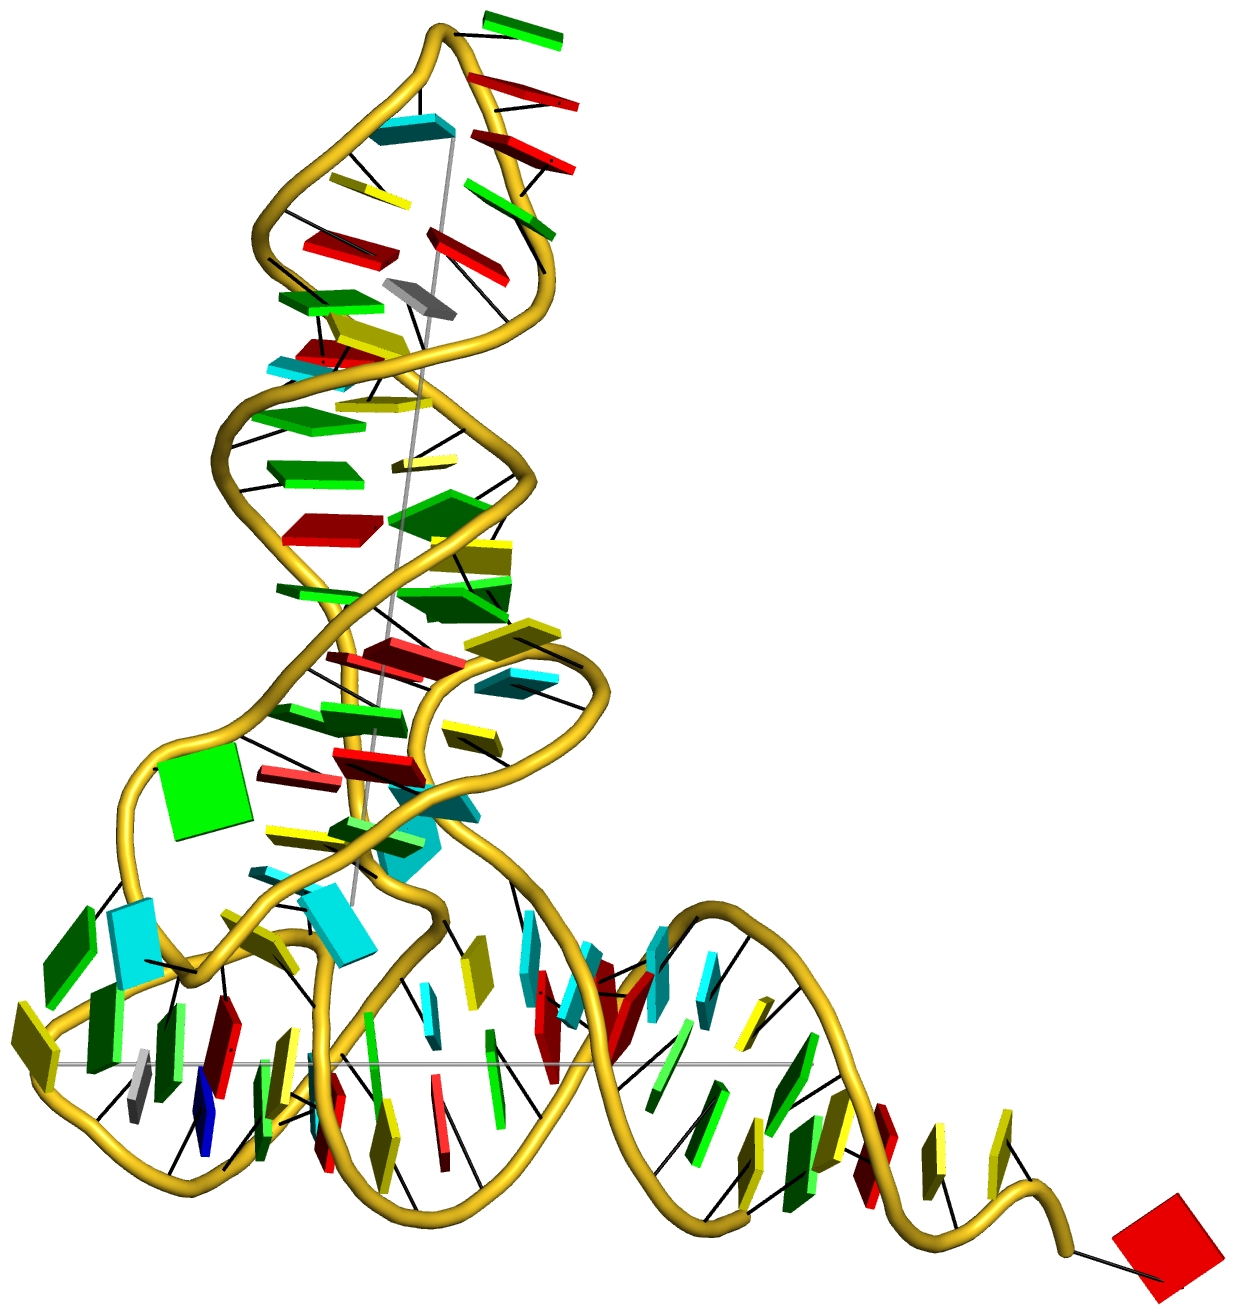
\includegraphics[width=0.9\textwidth]{RNA}
\end{figure}

Which came first: DNA to store genetic information, or proteins to catalyze reactions? RNA can do both, giving rise to the idea of the RNA World a selfish world in which each molecule looks after itself and grabs as much resource as it can.

\begin{figure}[H]
	\caption[Which came first: DNA or proteins?]{Which came first: DNA to store genetic information, or proteins to catalyze reactions?\cite{x3dna.org} DNA can be transcribed/translated to proteins, but some proteins are needed for this process. RNA can do both jobs: its structure allows the storage of genetic information and catalysis.}\label{TheRNAworld} 
	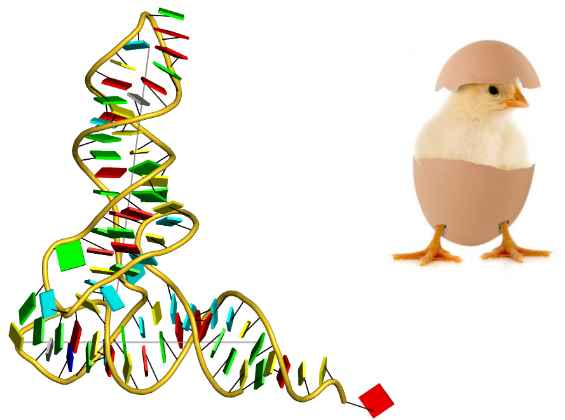
\includegraphics[width=0.9\textwidth]{TheRNAworld}
\end{figure}

Despite the attractiveness of this idea, nobody has been able to show that RNA can catalyze its own template-directed reproduction. However, some RNA molecules can catalyze the formation of other RNA from shorter fragments. They can form cooperative molecular networks, in which each catalyzes the formation of other RNAs.

The first example of such a mutually catalytic network
was constructed in the lab of Günter von Kiedrowski in Germany--Figure \ref{fig:MutualCatalysis1}. 
It consists of a cross-catalytic pair
of short nucleotide sequences.
The basic building blocks are
trimers A and B
that form each other's base-pair
complement.
\begin{itemize}
	\item The hexamers AA and BB now serve as templates
to which the complementary trimers can attach by forming base-pair bonds.
	\item For example, two B trimers can attach to an AA template, allowing the B trimers to ligate--or chemically join--into a fully formed BB hexamer.
	\item After strand separation, the original AA template is regained, plus a new BB template.
	\item In a similar way, such a BB template can facilitate the ligation of a new AA template from two A trimers.
\end{itemize}

\begin{figure}[H]
	\caption[Mutual Catalysis with Trimers A and B]{Mutual Catalysis with Trimers A and B, which form each other's complement\cite{patzke2007self}.}\label{fig:MutualCatalysis1}
	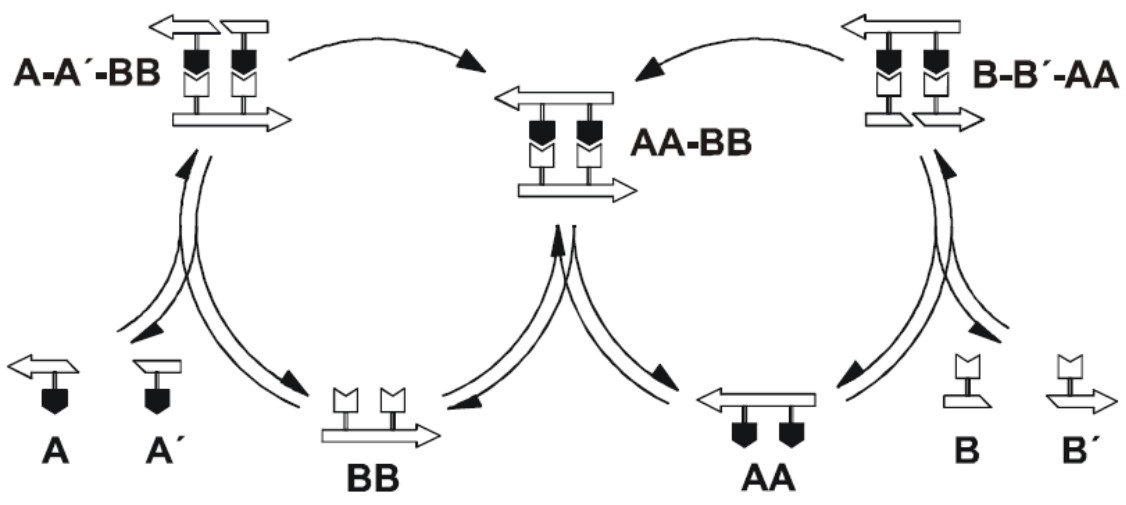
\includegraphics[width=0.8\textwidth]{MutualCatalysis1}
\end{figure}

More recently, an experimental system
with up to 16 RNA molecules,
each of around 200 nucleotides long
that mutually catalyzed each other's
formation from shorter fragments,
was created in the lab of Niles Lehman
at Portland State University--Figure \ref{fig:MutualCatalysis2}.

\begin{figure}[H]
	\caption[16 nucleotides that catalyze each other's formation]{16 nucleotides, around 16 base pairs each, that catalyze each other's formation}\label{fig:MutualCatalysis2}
	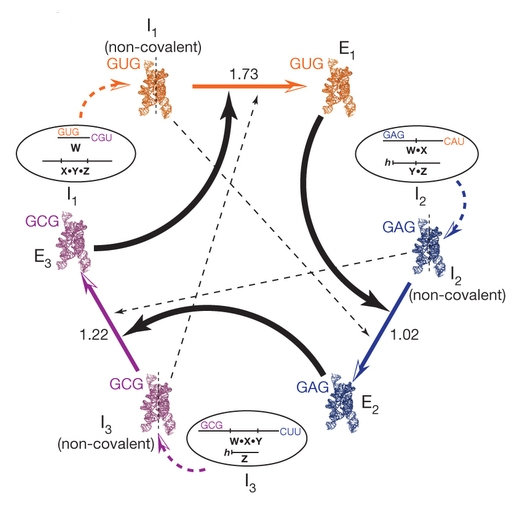
\includegraphics[width=0.8\textwidth]{MutualCatalysis2}
\end{figure}

However, such experimental systems are not restricted to RNA molecules.
A similar set of nine mutually catalytic peptides--or short proteins--was created and studied in detail by Gonen Ashkenasy and colleagues, then at the Scripps Research Institute--Figure \ref{fig:MutualCatalysis3}.

\begin{figure}[H]
	\caption[Mutual Catalysis with Peptides]{Mutual Catalysis with Peptides\cite{ashkenasy2004design}}\label{fig:MutualCatalysis3}
	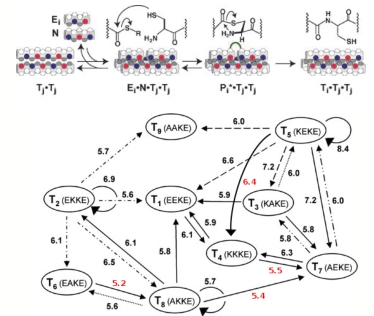
\includegraphics[width=0.9\textwidth]{MutualCatalysis3}
\end{figure}

What these experimental systems--Figures \ref{fig:MutualCatalysis1}, \ref{fig:MutualCatalysis2}, and \ref{fig:MutualCatalysis3}--
of mutually catalytic molecules
have in common is that
they are all instances
of an \gls{gls:autocatalytic:set}--Figure \ref{fig:AutoCatalytic1}.
An autocatalytic set is defined as
a set of reactions
and the molecules involved in them,
such that:
\begin{enumerate}
	\item Each reaction in the set is catalyzed
	by at least one of the molecules
	from the set itself
	and,
	\item Each molecule in the set
	can be produced
	from a basic food source
	through a sequence of reactions
	from the set itself
\end{enumerate}
The food source consists of
basic building blocks,
such as the RNA or peptide fragments
in the experimental examples,
or the molecules that were present
on the early Earth
in a purely prebiotic setting.
In other words, the food source
consists of those elements
that can be assumed to be available
in the environment.

Note that this concept of an autocatalytic set captures two essential properties of living systems.

\begin{itemize}
	\item all chemical reactions are facilitated and regulated by catalysts generated
	within the network itself. In other words, the system is catalytically closed.

	\item  it is self-sustaining from resources available in the environment.
\end{itemize}

\begin{figure}[H]
	\caption{An Autocatalytic Set}\label{fig:AutoCatalytic1}
	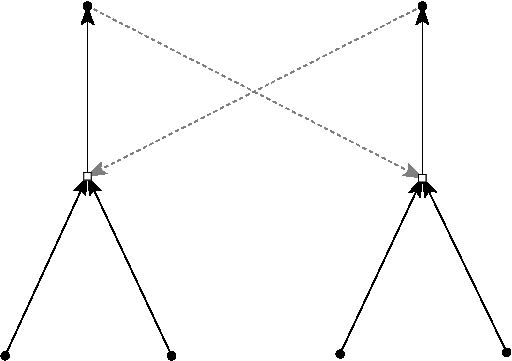
\includegraphics[width=0.9\textwidth]{AutoCatalytic1}
\end{figure}

Figure \ref{fig:AutoCatalytic2} shows a simple example
of an autocatalytic set formed by a reaction network where the molecule types--
the black dots--are represented by bit strings, that is, strings of zeros and ones.
The food source consists of
the monomers and dimers,
or bit strings of length one and two.
The longer molecules can be built up
through ligation reactions--
the white boxes--
between two shorter bit strings.
Solid black arrows indicate
reactants going into
and products coming out of
a ligation reaction,
and dashed gray arrows indicate which
molecules catalyze which reactions.
Given the definition
of an autocatalytic set,
it is easy to verify that this reaction
network satisfies its two properties.

Note that this simple example is similar to the experimental systems that have been constructed in the lab.
This concept of autocatalytic sets was originally introduced by Stuart Kaufmann, in descriptive form already back in 1971 and more formally in 1986.

More recently,
my colleague Mike Steel and myself
have done more detailed studies
of autocatalytic sets,
both mathematically
and computationally.
What these detailed studies have shown
is that autocatalytic sets
have a high probability of existing
in simple models
of chemical reaction networks--
also for chemically plausible
levels of catalysis.
For example,
in this simple bit string model--Figure \ref{fig:AutoCatalytic2}--
where catalysis is assigned randomly,
each molecule only needs to catalyze
between one and two ligation
reactions on average
to already have a high probability
of autocatalytic sets to exist
in random instances of the model.
Furthermore, it turns out that
autocatalytic sets
often consist of a hierarchy of smaller
and smaller autocatalytic subsets.
In other words,
a given autocatalytic set
often contains several smaller subsets
that themselves also form
autocatalytic sets.
For example,
this autocatalytic set of five reactions--Figure \ref{fig:AutoCatalytic2}--
contains two smaller
autocatalytic subsets -
one of two reactions
and one of three reactions.

\begin{figure}[H]
	\caption[Autocatalytic set 	with two smaller autocatalytic subsets]{This autocatalytic set of five reactions
		contains two smaller
		autocatalytic subsets\cite{hordijk2012structure}}\label{fig:AutoCatalytic2}
	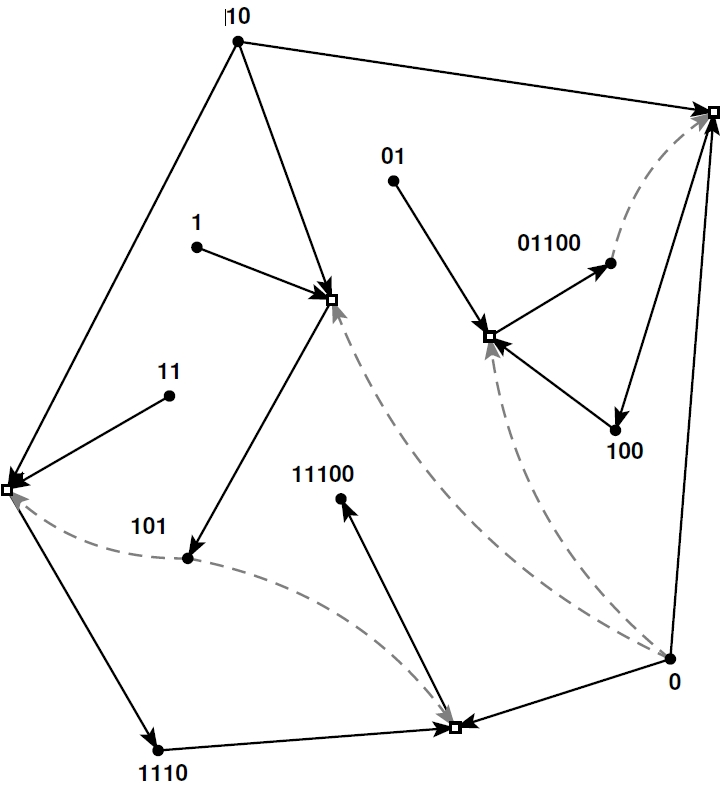
\includegraphics[width=0.9\textwidth]{AutoCatalytic2}
\end{figure}

Figure \ref{fig:AutoCatalyticSubsets} is another example from the same bit string model,
which shows an autocatalytic set of eight reactions containing various smaller autocatalytic subsets, as indicated by the differently colored shapes.
This hierarchical subset structure can enable the existence of different types of \glspl{gls:protocell}.

\begin{figure}[H]
	\caption[An Autocatalytic Set made up of Autocatalytic Subsets]{An Autocatalytic Set made up of Autocatalytic Subsets\cite{hordijk2017chasing}}\label{fig:AutoCatalyticSubsets}
	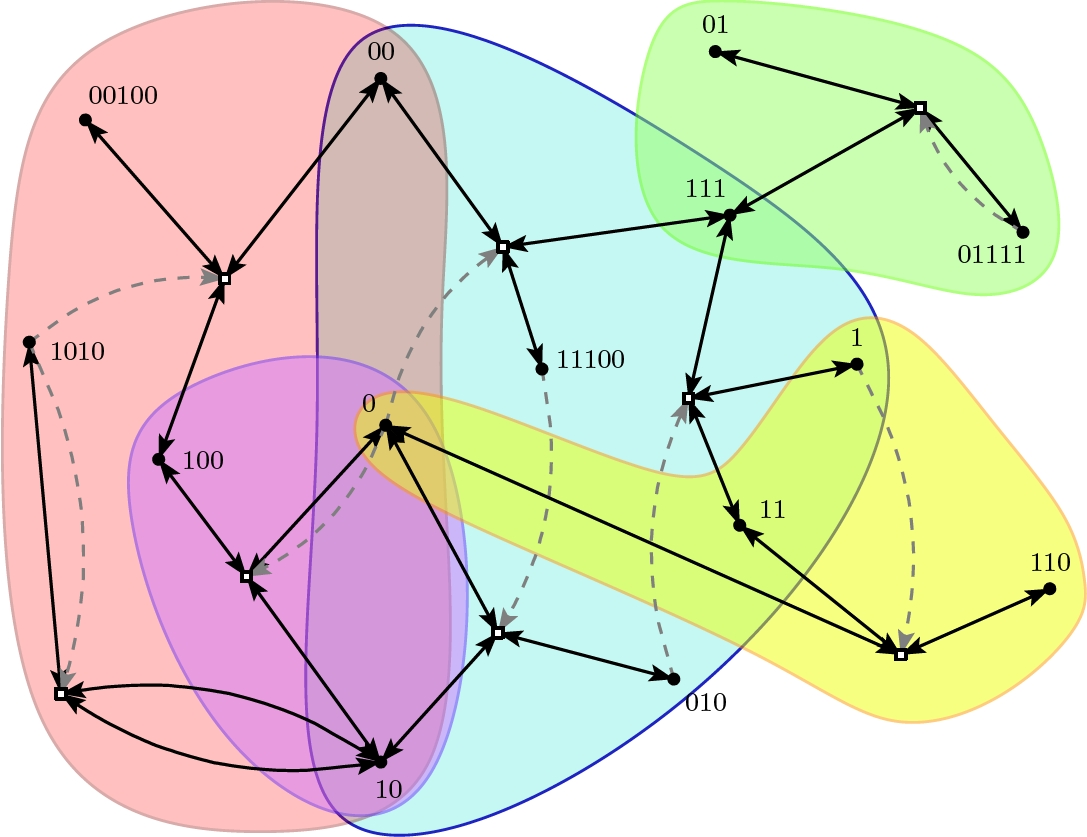
\includegraphics[width=0.9\textwidth]{AutoCatalyticSubsets}
\end{figure}

Imagine two compartments formed, for example, by lipid membranes, which have been shown to form, grow and divide spontaneously under appropriate circumstances.
Now, assume that the same chemistry can take place in both of these compartments, but in one of them only the red autocatalytic subset is currently present, and in the other one
only the blue autocatalytic subset.
This would form two different types of \glspl{gls:protocell}, which might compete with each other for food resources--in this case the monomers and dimers--and perhaps even give rise to some simple evolutionary dynamics.



Computational studies have shown
that autocatalytic sets
are indeed able to evolve
and become more complex over time,
exactly because of this existence
of multiple autocatalytic subsets.
This is shown in Figure \ref{fig:EvolveableProtocells} with simulated
\glspl{gls:protocell} changing color over time,
depending on which autocatalytic
subsets they contain.
These results are mostly based on
computational models
of chemical reaction networks
such as the Bitstream model.
However, the formal autocatalytic
sets framework
has also been used to study
and understand
the existing experimental networks
in more detail,
both the RNA one and the peptide one.

\begin{figure}[H]
	\caption[Computational studies of autocatalytic sets]{Computational studies have shown
		that autocatalytic sets	
		are indeed able to evolve
		and become more complex over time\cite{hordijk2018population}}\label{fig:EvolveableProtocells}
	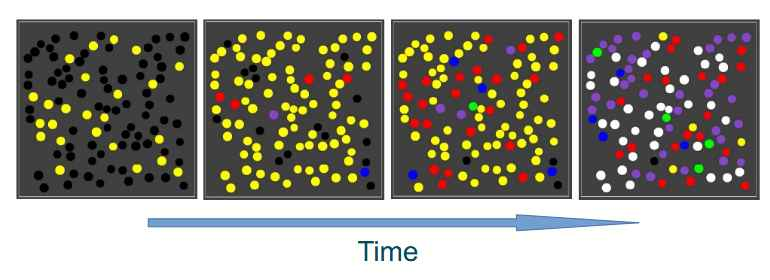
\includegraphics[width=0.8\textwidth]{EvolveableProtocells}
\end{figure}

Moreover, we have shown that the metabolic network of \emph{E.coli} forms a large autocatalytic set--Figure \ref{fig:AutoCatalyticEcoli}.
This supports the original claim
that autocatalytic sets capture
essential properties of living systems,
in particular the catalytic closure
and self-sustainability.
So, autocatalytic sets are not just
abstract mathematical constructs,
but they do exist in real chemical
and biological reaction networks
and can be studied formally
within those systems.
\begin{figure}[H]
	\caption[The metabolic network of \emph{E.coli}
	forms a large autocatalytic set.]{The metabolic network of \emph{E.coli}
		forms a large autocatalytic set\cite{sousa2015autocatalytic}}\label{fig:AutoCatalyticEcoli}
	\includegraphics[width=\textwidth]{AutoCatalyticEcoli}
\end{figure}

In conclusion, given that autocatalytic
sets are highly likely to exist
in simulated chemical reaction networks,
that they are able to evolve
and become more complex,
and that they actually exist
in real chemical and biological
networks as well,
an alternative scenario emerges
for a possible origin of life--Figure \ref{fig:CooperativeOrigin}.
Perhaps life started
with the spontaneous formation
of one or more autocatalytic sets,
which then gradually... diversified
and evolved into more and more
complex chemical networks,
eventually leading to
true metabolic networks.
In other words,
life arising as a cooperative effort
among diverse molecule types
and catalytically closed
and self-sustaining
chemical reaction networks.
I believe there is grandeur
in this view of the origin of life.

\begin{figure}[H]
	\caption[Life arising as a cooperative effort
	among diverse molecule types]{Life arising as a cooperative effort
		among diverse molecule types
		and catalytically closed
		and self-sustaining
		chemical reaction networks}\label{fig:CooperativeOrigin}
	\includegraphics[width=\textwidth]{CooperativeOrigin}
\end{figure}

References: \cite{wim2017origin,wim2019wandering,hordijk2012structure,sousa2015autocatalytic}

\subsection[Reaction Networks and Autocatalysis]{Reaction Networks and Autocatalysis--Nathaniel Virgo}

\subsubsection{Autocatalysis}

\Gls{gls:autocatalysis} is chemical self-production: \glsdesc{gls:autocatalysis}. Why is it important? The ability to make more of itself is a key feature of all living systems, even those that don't reproduce--Figure \ref{fig:LifeMakesLife}. And do the question naturally arises: under what circumstances can this chemical self production occur in an a-biological system? Answering this is important for several reasons.\begin{itemize}
	\item  It helps us to answer questions about the origin of metabolism: how did the molecules of life first get created before there was life to make them?
	\item It also help us to answer questions about the origin of evolution: how did cells acquire the ability to produce not just more cells in general, but mroe of its own species with its own genetic make-up?
\end{itemize}
\begin{figure}[H]
	\begin{center}
		\caption{Life Makes Life}\label{fig:LifeMakesLife}
		\includegraphics[width=0.8\textwidth]{LifeMakesLife}
	\end{center}
\end{figure}

The place to start is by thinking about chemical reactions. Figure \ref {fig:ChemicalReaction} illustrates the raction $2A \rightarrow B$.

\begin{figure}[H]
	\caption{Chemical Reaction: $2A \rightarrow B$}\label{fig:ChemicalReaction}
	\begin{subfigure}[m]{0.45\textwidth}
		\caption{We have a whole lot of molecules $A$ rushing around}
		\includegraphics[width=\textwidth]{ChemicalReaction1}
	\end{subfigure}
	\begin{subfigure}[m]{0.45\textwidth}
		\caption{When two $A$s  collide they form $B$}
		\includegraphics[width=\textwidth]{ChemicalReaction2}
	\end{subfigure}
\end{figure}

Reactions generally happen faster the higher the concentration of reactants. One type of reaction that particularly interests us is catalysis, which is crucial in biology: it is what enzymes do.
\begin{align*}
	2A \xrightarrow{\text{C}}& B \text{, or}\\
	2A + C \rightarrow& B +C \text{, if we prefer to think of $C$ as a product.}
\end{align*}

We will work through one example, which will serve as out first reaction network.

\begin{align*}
	2A + C \rightarrow& C2A \\
	C2A \rightarrow& CB\\
	CB \rightarrow& B + C \text{, so the nett reaction is:}\\
	2A + C \rightarrow& B+C
\end{align*}
There are many ways to draw this as a reaction network. Figure \ref{fig:CatalysisReactionNetwork} is a simple example. The catalytic cycle is a common feature in reaction networks.

\begin{figure}[H]
	\caption{Catalysis as a reaction network, with \gls{gls:catalyst} C}\label{fig:CatalysisReactionNetwork}
	\includegraphics[width=0.9\textwidth]{CatalysisReactionNetwork}
\end{figure}

\Gls{gls:reaction-network}: \glsdesc{gls:reaction-network}. Our first example is the Formose Reaction--Figure \ref{fig:Formose}, which is a way to convert formaldehyde to sugars. Here the key point it is autocatalytic.

\begin{figure}[H]
	\caption[The Formose Reaction]{The Formose Reaction\cite{andersen2013generic}}\label{fig:Formose}
	\includegraphics[width=0.9\textwidth]{Formose}
\end{figure}

Figure \ref{fig:formose:simplified} shows a simplified version of the formose reaction.
\begin{figure}[H]
	\caption{The Formose Reaction(simplified)}\label{fig:formose:simplified}
	\begin{subfigure}[h]{0.45\textwidth}
		\caption{First step: two molecules of formaldehyde fuse to acetaldehyde.}
		\includegraphics[width=\textwidth]{FormoseStep1}
	\end{subfigure}
	\begin{subfigure}[h]{0.45\textwidth}
		\caption{For simplicity let's suppress every thing except carbon.}
		\includegraphics[width=\textwidth]{FormoseStep1A}
	\end{subfigure}
	\begin{subfigure}[h]{0.45\textwidth}
		\caption{Once you have two carbons it is quickly converted to 3}
		\includegraphics[width=\textwidth]{FormoseStep2}
	\end{subfigure}
	\begin{subfigure}[h]{0.45\textwidth}
		\caption{Then to 4. It can continue to grow, and to branch.}
		\includegraphics[width=\textwidth]{FormoseStep3}
	\end{subfigure}
	\begin{subfigure}[h]{0.45\textwidth}
		\caption{Alternatively it can split in to two 2 carbon molecules.}
		\includegraphics[width=\textwidth]{FormoseStep4}
	\end{subfigure}
	\begin{subfigure}[h]{0.45\textwidth}
		\caption{And the cycle repeats.}
		\includegraphics[width=\textwidth]{FormoseStep5}
	\end{subfigure}
\end{figure}

 Graphically the process looks like Figure \ref{fig:Formose1}. Figure \ref{fig:Formose2} shows the speed of the reaction: initially there very little $C_2$, but the branching step produces more (exponentially), until the reaction saturates.  
 
\begin{figure}[H]
	\begin{subfigure}[t]{0.45\textwidth}
		\caption{The Formose Reaction as an autocatalytic cycle with branching step}\label{fig:Formose1}
		\includegraphics[width=\textwidth]{Formose1}
	\end{subfigure}
	\begin{subfigure}[t]{0.5\textwidth}
		\caption{Sugar concentration versus time.}\label{fig:Formose2}
		\includegraphics[width=\textwidth]{Formose2}
	\end{subfigure}
\end{figure}

 Autocatalysis is a very active area of experimental research. One example is biological metabolites, or substances that may have played similar roles, such as the reverse citric acid cycle, which is important to most autotrophs. 

\begin{itemize}
	\item Reverse citric acid cycle--Figure \ref{fig:ReverseCitricAcidCycle}
	\item Key part of metabolism of many organisms (autotropha), but 
	\item unlike formose, many steps are difficult reactions, requiring specific catalysts
\end{itemize}

\begin{figure}[H]
	\caption{Reverse Citric Acid Cycle}\label{fig:ReverseCitricAcidCycle}
	\includegraphics[width=0.9\textwidth]{ReverseCitricAcidCycle}
\end{figure}

\subsubsection{Autocatalysis vs biological replication}

At first sight these are similar, but replication exhibits diversity that is inherited--Figure \ref{fig:AutoCatalysisVsRepl}.

\begin{figure}[H]
	\caption{Autocatalysis vs biological replication}\label{fig:AutoCatalysisVsRepl}
	\begin{subfigure}[t]{0.45\textwidth}
		\caption{Autocatalysis}
		\includegraphics[width=\textwidth]{AutoCatalysisRepl1}
	\end{subfigure}
	\begin{subfigure}[t]{0.45\textwidth}
		\caption{Biological Replication:there is diversity in bilogy, and that tends to be inherited.}
		\includegraphics[width=\textwidth]{AutoCatalysisRepl2}
	\end{subfigure}
\end{figure}

One solution is Template Regulators--Figure \ref{fig:TemplateReplicators}. 

\begin{figure}[H]
	\caption[Template Regulators]{Template Regulators\cite{von1986self,virgo2012evolvable}}\label{fig:TemplateReplicators}
	\begin{subfigure}[t]{0.45\textwidth}
		\caption{First step}
		\includegraphics[width=\textwidth]{TemplateReplicators1}
	\end{subfigure}
	\;\;
	\begin{subfigure}[t]{0.45\textwidth}
		\caption{String has been copied}
		\includegraphics[width=\textwidth]{TemplateReplicators2}
	\end{subfigure}
	\begin{subfigure}[t]{0.45\textwidth}
		\caption{Two separate copies}
		\includegraphics[width=\textwidth]{TemplateReplicators3}
	\end{subfigure}
	\;\;
	\begin{subfigure}[t]{0.45\textwidth}
		\caption{Modified RNA timers as replicators\cite{von1986self}. Main problem: the monomers have to be quite complicated to avoid side reactions.}
		\includegraphics[width=\textwidth]{TemplateReplicators4}
	\end{subfigure}
\end{figure}


This brings us to Eigen's paradox Figure \ref{fig:EigensParadox} \cite{eigen1971selforganization} \cite{wiki:error-threshold}.
\begin{itemize}
	\item Without error correction enzymes, the maximum size of a replicating molecule is about 100 base pairs.
	\item For a replicating molecule to encode error correction enzymes, it must be substantially larger than 100 bases.
\end{itemize}

 
\begin{figure}[H]
	\caption[Eigen's Paradox]{If you look at DNA replication in the cell, it is quite a complex process. To get the complicated machines you need natural selection; to get natural selection you need high fidelity reproduction, hence the complicated machinery.}\label{fig:EigensParadox}
	\includegraphics[width=0.9\textwidth]{EigensParadox}
\end{figure}

We need to think of simpler mechanisms for heredity than are now used in the cell.
\begin{itemize}
	\item Template replication
	\item  Replicase-like RNAzyme that can copy itself
	\begin{itemize}
		\item similar issue: the molecule has to be quite complex
		\item it’s a promising area of active study.
	\end{itemize}
	\item Compositional heredity - no heteropolymers, 	information stored in composition of \gls{gls:protocell} instead\cite{vasas2012evolution,segre2000compositional}.
\end{itemize}

\subsubsection{Summary}

\begin{itemize}
	\item Autocatalysis is chemical self-production
	\item Reaction networks are a useful tool to understand it
	\item Replication with heredity is more difficult than autocatalysis
	\item Open questions:
	\begin{itemize}
		\item  How can biomolecules be produced abiotically?
		\item Did the first autocatalytic cycles resemble biochemistry,
		or were they completely different?
		\item How did evolution by natural selection first arise?
	\end{itemize}
\end{itemize}

See also   \cite{carnall2010mechanosensitive,king1977symbiosis,king1982recycling,szathmary2000evolution,virgo2016complex}


\section{Evolutionary Theory}

We will talk about the evolutionary theory of the origin of life.

\subsection[An Introduction]{An Introduction-- Michael Travisano}

There's really three important processes--Figure \ref{fig:EvolutionaryOrigin}.

\begin{itemize}
	\item Metabolism--Figure \ref{fig:EvolutionaryOrigin1}
	\item Genetic Transmission--Figure \ref{fig:EvolutionaryOrigin2}
	\item Evolution--Figure \ref{fig:EvolutionaryOrigin3}
\end{itemize}

\begin{figure}[H]
	\caption{Evolutionary origin of three processes}\label{fig:EvolutionaryOrigin}
	\begin{subfigure}[t]{0.3\textwidth}
		\caption{Metabolism: organism eats things, digests them, and gets rid of waste products.}\label{fig:EvolutionaryOrigin1}
		\includegraphics[width=\textwidth]{EvolutionaryOrigin1}
	\end{subfigure}
	\;\;
	\begin{subfigure}[t]{0.3\textwidth}
		\caption{Genetic Transmission: organism replicates itself, and transmits genes to an offspring.}\label{fig:EvolutionaryOrigin2}
		\includegraphics[width=\textwidth]{EvolutionaryOrigin2}
	\end{subfigure}
	\;\;
	\begin{subfigure}[t]{0.3\textwidth}
		\caption{Evolution: transmits not-exactly itself.}\label{fig:EvolutionaryOrigin3}
		\includegraphics[width=\textwidth]{EvolutionaryOrigin3}
	\end{subfigure}
\end{figure}

These processes are what we think about the evolutionary origin. It is challenging if we think of them as they are in life today.

\subsubsection{Metabolism}

Metabolic pathways are complex. The Citric Acid Cycle--Figure \ref{fig:CitricAcidCycle}--is very complex, with many steps \& many enzymes; it is super well ordered. It is hard to imagine how we could go from nothing to Figure \ref{fig:CitricAcidCycle}.

\begin{figure}[H]
	\caption{The citric acid cycle: metabolic pathways are complex}\label{fig:CitricAcidCycle}
	\includegraphics[width=0.9\textwidth]{CitricAcidCycle}
\end{figure}

 What probably happened is you didn't go from nothing to  Figure \ref{fig:CitricAcidCycle}.  There are many non-living ''metabolism-like'' processes on Earth, such as the Black Smoker--Figure \ref{fig:BlackSmoker}. We don't know which one was the most important.
 
\begin{figure}[H]
	\caption[Black Smoker]{Black Smoker: one of the many non-living metabolism-like processes on Earth}\label{fig:BlackSmoker}
	\includegraphics[width=0.9\textwidth]{BlackSmoker}
\end{figure}

\subsubsection{Genetic Transmission}

DNA replication is complicated nowadays--Figure \ref{fig:DNA_replication_complex}--it has all these steps. And this is only the most simple part of transmission: it doesn't include meiosis or any of the other steps in reproduction. It is difficult to see how we went from nothing to all the modern complexity, so that is probably not what happened.
\begin{figure}[H]
	\caption{DNA replication is complex}\label{fig:DNA_replication_complex}
	\includegraphics[width=0.9\textwidth]{DNA_replication_complex}
\end{figure}

We can see that if we take the precursors of DNA and RNA and put them in water, ehay will self assemble into things that can carry information--Figure \ref{fig:SpontaneousFormation}. 
\begin{figure}[H]
	\caption[Spontaneous formation and base pairing]{Spontaneous formation and base pairing of plausible prebiotic nucleotides in water\cite{cafferty2016spontaneous}}\label{fig:SpontaneousFormation}
	\includegraphics[width=0.9\textwidth]{SpontaneousFormation}
\end{figure}

\subsubsection{Evolution of Evolution}

This is perhaps the most challenging of all. DNA replication is complex, and must be evolvable. Genetic Transmission must be sensitive enough to mutations for it to have an effect, but not too sensitive, so it doesn't break--Figure \ref{fig:EvolutionOfEvolution}.
\begin{figure}[H]
	\caption{DNA replication is complex and must be evolvable}\label{fig:EvolutionOfEvolution}
	\includegraphics[width=0.9\textwidth]{EvolutionOfEvolution}
\end{figure}

We know that there were precursors to modern day heritable material probably around at the origin of life--Figure \ref{fig:SpontaneousFormation}. Could they change and still work? Yes: they mutate, and work in different ways--Figure \ref{fig:ContinuityInEvolution}.

\begin{figure}[H]
	\caption[Continuity in Evolution: On the Nature of Transitions]{Continuity in Evolution: On the Nature of Transitions\cite{fontana1998continuity}}\label{fig:ContinuityInEvolution}
	\includegraphics[width=0.9\textwidth]{ContinuityInEvolution}
\end{figure}

There are precursors for all the mechanisms we need. The big challenge is putting them together.
\begin{itemize}
	\item Preexisting Metabolism
	\item Simple Genetic Transmission
	\item Evolution in Simple Life
\end{itemize}

Suggested Reading
\begin{itemize}
	\item \cite{maynard1999origins} covers origins of life, eukaryotes, sex, society; 
	\item \cite{sumper1975evidence} treats life more mechanistically, and shows how we can use chemistry to understand it.
\end{itemize}

See also \cite{eigen1971selforganization,orgel2004prebiotic,kun2005real,ratcliff2014experimental}.

\subsection[A Recipe for Adaptation]{A Recipe for Adaptation-- David Baum}

Since the capacity for Adaptive Evolution is central to almost any definition of life, we need to understand what is the simplest system capable of undergoing adaptive evolution. Life is too complex to explain without an adaptive
process\cite{hoyle1983intelligent}--Figure \ref{fig:LifeTooComplex}. A cell is too complicated to  just emerge, so we need to think about:

\begin{itemize}
	\item  how does adaptation work?
	\item could start working on something simpler than a modern cell?
\end{itemize}.

\begin{figure}[H]
	\caption{Life is too complex to explain without an adaptive
		process!}\label{fig:LifeTooComplex}
	\includegraphics[width=0.9\textwidth]{LifeTooComplex}
\end{figure}

Figure \ref{fig:ReplicationMutationSelection} is a reminder of the way Darwinian Evolution works. Favoured variant \textit{could} be more complex, but it doesn't need to be. Natural selection \emph{can} yield greater complexity, but it doesn't have to.
\begin{figure}[H]
	\caption[Darwinian evolution: Replication--Mutation--Selection]{Darwinian evolution: Replication--Mutation--Selection. We start with a bacterium, which gives rise to two daughter cells. The DNA which it gives to the daughters controls the features of those cells. The DNA at the top left might have a mutation--red dot--which allows it to function differently, which \emph{might} allow its descendants to outcompete those that weren't mutated.}\label{fig:ReplicationMutationSelection}
	\includegraphics[width=0.9\textwidth]{ReplicationMutationSelection}
\end{figure}

To get to the first cell we need some process of natural selection that could allow it to complexify.
 But, if you need cells and a genetic system to evolve adaptively it is hard to see how life can start--Figure \ref{fig:ChickenEgg}.
\begin{figure}[H]
	\caption[If you need cells and a genetic system to evolve adaptively...]{If you need cells and a genetic system to evolve adaptively it is hard to see how life can start}\label{fig:ChickenEgg}
	\begin{subfigure}[t]{\textwidth}
		\caption{To get to the first cell we need some process of natural selection that could allow it to complexify}
		\includegraphics[width=0.9\textwidth]{ChickenEgg}
	\end{subfigure}
	\begin{subfigure}[t]{0.45\textwidth}
		\caption{What is required for Natural Selection?--Replication.}
		\includegraphics[width=0.9\textwidth]{ChickenEgg1}
	\end{subfigure}
	\;\;\;\;\;\;
	\begin{subfigure}[t]{0.45\textwidth}
		\caption{The only process of replication that we know about today, that cells use, is a very complicated process.}
		\includegraphics[width=0.9\textwidth]{ChickenEgg2}
	\end{subfigure}
\end{figure}

Scientists have figured out a few ways out of this.

\begin{itemize}
	\item Cells could pass on their identity by passing on a
	dynamically maintained chemical state (analog)--Figure \ref{fig:CellWithoutGenes}.
	\item Self-replicating molecules could give rise to cells--Figure \ref{fig:GenesWithoutCells}.
\end{itemize}

\begin{figure}[H]
	\caption[Cells without genes]{Cells without genes: cells could pass on their identity by passing on a dynamically maintained chemical state }\label{fig:CellWithoutGenes}
	\includegraphics[width=0.9\textwidth]{CellWithoutGenes}
\end{figure}

\begin{figure}[H]
	\caption[Genes without cells]{Genes without cells: Self-replicating molecules could give rise to cells}\label{fig:GenesWithoutCells}
	\includegraphics[width=0.9\textwidth]{GenesWithoutCells}
\end{figure}

Many people, including David Baum, are concerned that this is still too complex. The simplest \gls{gls:protocell} capable of dividing, and enclosing this dynamical system would still have to be pretty complicated.
\begin{itemize}
	\item It would have to arise spontaneously without any prior adaptive process;
	\item it would need to be able to grow, regulate the transport of metabolites into and out of the cell;
	\item it would have to be able to divide
\end{itemize}
 That seems unlikely to arise spontaneously. A single \gls{gls:RNA} molecule is unlikely to arise spontaneously. Nucleotides are not likely to be sitting around in the environment in high abundance.

So some scientists have begun looking around for something simpler. 
One possibility is no genetics and no cells. Adaptive material is possible if material in some sort of spatial structure--Figure \ref{fig:WangWang}.

\begin{figure}[H]
	\caption[Spatial structure does not require bounded cells]{Spatial structure does not require bounded cells\cite{wang2015evolution}}\label{fig:WangWang}
	\includegraphics[width=0.9\textwidth]{WangWang}
\end{figure}

Perhaps the first adaptive evolving systems were flat living systems--Figure \ref{fig:Baum2018}--slime-like things that lived on surfaces, had a metabolism, maintained a dynamics state, that could grow and evolve adaptively, and later give rise to cells. A cell can be seen as a very good way for a surface dweller to get to another surface--Figure \ref{fig:Baum2018}. One can imagine a situation in which, in an ancient ocean, there were minimal surfaces coated with life-like systems that could grow, spread, and be subjected to selection.

\begin{figure}[H]
	\caption[A very good way for a surface dweller to get to another surface]{ A cell can be seen as a very good way for a surface dweller to get to another surface\cite{baum2018origin}}\label{fig:Baum2018}
	\includegraphics[width=0.9\textwidth]{Baum2018}
\end{figure}

Cells could have started as a transport mechanism--Figure \ref{fig:Baum2015}--which enable certain types to spread.

\begin{figure}[H]
	\caption[Cells could have started as a transport mechanism]{Adaptive evolution started before cells or genetics: cells could have started as a transport mechanism\cite{baum2015selection}}\label{fig:Baum2015}
	\includegraphics[width=0.9\textwidth]{Baum2015}
\end{figure}

To summarize:
\begin{itemize}
	\item Evolutionary theory plays a central role--Figure \ref{fig:Baum2018a};
	\item  Evolutionary theory is a constantly changing field, and our models have become more and more sophisticated;
	\item we now appreciate that a view of Evolution that requires cells and genetic encoding is perhaps too stringent;
	\item it is becoming clear that advances in the origin of life field may come from appreciating the fact that very simple systems, much simpler than we are used to thinking about, could be the first evolving progenitors of life as we know it.
\end{itemize}


\begin{figure}[H]
	\caption[Evolutionary theory plays a central role]{Evolutionary theory plays a central role\cite{baum2018origin}}\label{fig:Baum2018a}
	\includegraphics[width=0.9\textwidth]{Baum2018a}
\end{figure}

References: \cite{hoyle1983intelligent,wang2015evolution,baum2018origin,baum2015selection}.

\subsection[Chance \& Change]{Chance \& Change--Andrew Rominger}

\subsubsection{Introduction: Definition of Evolution}

\Gls{gls:evolution} is a theory of chance events, and change through time. For this course it is defined in Figure \ref{fig:ChangeThroughTime}.
\begin{figure}[H]
	\caption[Evolution]{\Gls{gls:evolution}: \glsdesc{gls:evolution}}\label{fig:ChangeThroughTime}
	\includegraphics[width=0.9\textwidth]{ChangeThroughTime}
\end{figure}

We will be talking about the 4 key processes that make evolution possible, and perspectives on origins--\gls{gls:LUCA} and the complexity of life.

\subsubsection{4 key processes that make evolution possible}

\begin{itemize}
	\item Reproduction (+ heritability)--Figure \ref{fig:Reproduction1}
	\begin{itemize}
		\item can ignore haploid/diploid if mating random
		\item resources are finite $\implies$ maximum population size is finite
		\item $\implies$ after a certain number of generations, everything that is alive can be traced back to a single ancestor--Figure \ref{fig:Coalescence}. This is called ''coalescence''.
		\item Coalescence theory allows us to make simple mathematical predictions that are very powerful
		\begin{itemize}
			\item The probability of two individuals having a common ancestor one generation back is $\frac{1}{N}$
			\item The probability of two individuals not having a common ancestor one generation back is $1-\frac{1}{N}$
			\item The probability of two individuals having a common ancestor precisely $t$ generations back is $P_c(t)=\frac{1}{N}\big(1-\frac{1}{N}\big)^{t-1}$
			\item For a very large population $\lim\limits_{N\rightarrow \infty} P_c(t)=\frac{1}{N}e^{-\frac{t-1}{N}}$
			\item Because Earth is finite and very old, \gls{gls:LUCA} is less an
			indication of the singularity of life’s origin and more a
			statistical artifact related to ''Gambler’s ruin''
		\end{itemize}
	
	\end{itemize}
	\item Mutation: this is how we get variation in a population. Figure \ref{fig:Mutation1} shows the substitution of a new base pair into the genetic sequence. It is very rare, but it is important. There are other sources of variation:
	\begin{itemize}
		\item  Insertion;
		\item Deletion;
		\item Inversion
		\item Recombination;
		\item Migration
	\end{itemize}
	These all depend on mutation to create variation in the first place.

	\item Drift. This occurs when the new mutant doesn't have an advantage over the un-mutated form--Figure \ref{fig:Neutral}. It might die out, or it might drift to a higher frequency in the population. The probability of it becoming fixed is  $\frac{1}{N}$.
	
	\item Selection--The fate of mutations with fitness consequences--Figure \ref{fig:Selection}. \Gls{gls:fitness} is \glsdesc{gls:fitness}. The probability of a beneficial mutation becoming fixed is higher than that of a neutral one, and the probability of it being lost is correspondingly lower.

\end{itemize}

\begin{figure}[H]
	\caption[Reproduction (+ heritability)]{Reproduction (+ heritability): Offspring inherits parent’s traits}\label{fig:Reproduction1}
	\includegraphics[width=0.8\textwidth]{Reproduction1}
\end{figure}

\begin{figure}[H]
	\caption[Coalescence]{Populations are finite $\implies$ after a certain number of generations, everything that is alive can be traced back to a single ancestor.}\label{fig:Coalescence}
	\includegraphics[width=0.9\textwidth]{Coalescence}
\end{figure}

\begin{figure}[H]
	\caption[Mutation]{Mutation: the substitution of a new base pair into the genetic sequence.}\label{fig:Mutation1}
	\includegraphics[width=0.8\textwidth]{Mutation1}
\end{figure}

\begin{figure}[H]
	\caption{The fate of mutations without fitness
		consequences}\label{fig:Neutral}
	\includegraphics[width=0.9\textwidth]{Neutral}
\end{figure}

\begin{figure}[H]
	\caption{The fate of mutations with fitness
		consequences}\label{fig:Selection}
	\begin{subfigure}[t]{0.4\textwidth}
		\includegraphics[width=0.9\textwidth]{Mutation2}
	\end{subfigure}
	\begin{subfigure}[t]{0.55\textwidth}
		\includegraphics[width=0.9\textwidth]{Selection}
	\end{subfigure}
\end{figure}

\subsubsection{Mutation Space}

This is a more interesting an nuanced view of selection and drift.
Figure \ref{fig:MutationSpace} depicts \textit{Mutation Space}, a network of sequences connected by edges of single base-pair mutations.
\begin{figure}[H]
	\caption[Mutations and sequence spaces]{Mutations and sequence spaces:  a network of sequences connected by edges of single basepair mutations}\label{fig:MutationSpace}
	\includegraphics[width=0.9\textwidth]{MutationSpace}
\end{figure}

 Over this space we can overlay a Fitness Landscape--Figure \ref{fig:FitnessLandscapeMovement}. Notice that probability of a mutation \textit{does not depend on fitness}, but the fate of the mutation does.
 
\begin{figure}[H]
	\caption{Over this space we can overlay a Fitness Landscape}\label{fig:FitnessLandscapeMovement}
	\includegraphics[width=0.9\textwidth]{FitnessLandscapeMovement}
\end{figure}

It is obvious that life has differing levels of complexity--Figure \ref{fig:FitComplex}. At first blush is might seem that more complex organisms are somehow fitter--Figure \ref{fig:FitComplex1}, but this is far from universally true--Figure \ref{fig:FitComplex2}. Organizations that are very different in complexity are likely very different species--Figure \ref{fig:FitComplex3}. Everything that we have said about fitness applies only within a single population; the idea of fitness across species is very controversial. A priori any relation between fitness and species is \emph{possible}--increasing, decreasing, flat--Figure \ref{fig:FitComplex4}.
 This leaves an open question: why did life become more complex? The answer possibly involves an entropic exploration of sequence space, some more complex, other less so. Maybe just a random walk?

\begin{figure}[H]
	\caption{Fitness and Complexity}\label{fig:FitComplex}
	\begin{subfigure}[t]{0.45\textwidth}
		\caption{At first blush is might seem that more complex organisms are somehow fitter}\label{fig:FitComplex1}
		\includegraphics[width=\textwidth]{FitComplex1}
	\end{subfigure}
	\begin{subfigure}[t]{0.45\textwidth}
		\caption{But this is far from universally true}\label{fig:FitComplex2}
		\includegraphics[width=\textwidth]{FitComplex2}
	\end{subfigure}
	\begin{subfigure}[t]{0.45\textwidth}
		\caption{Organizations that are very different in complexity are likely very different species}\label{fig:FitComplex3}
		\includegraphics[width=\textwidth]{FitComplex3}
	\end{subfigure}
	\begin{subfigure}[t]{0.45\textwidth}
		\caption{ A priori any relation between fitness and species is \emph{possible}}\label{fig:FitComplex4}
		\includegraphics[width=\textwidth]{FitComplex4}
	\end{subfigure}
\end{figure}


\subsubsection{Real World Complexities}.

\begin{itemize}
	\item  Fluctuating population sizes
	\item  Non-random mating (random mating allowed us to avoid considering diploids)
	\item  Fluctuating environments and variable selection
\end{itemize}

These complexities are probably good, because they help answer the question if Figure \ref{fig:RealWorldComplexities}: how to cross a valley in the fitness landscape?
\begin{figure}[H]
	\caption{Real World Complexities: how to cross a valley?}\label{fig:RealWorldComplexities}
	\includegraphics[width=0.9\textwidth]{RealWorldComplexities}
\end{figure}

Further reading: \cite{gillespie1984molecular,kauffman1989nk,kimura1983neutral,kingman2000origins,patwa2008fixation,poelwijk2007empirical,rosenberg2002genealogical}.

\section[Niche Construction]{Niche Construction--Michael Travisano}

Environments can be harsh, as Figure \ref{fig:Harsh1} shows, but living organisms can alter their environments, often for the better. Pioneer species break up the ground and allow others to colonize--Figures \ref{fig:Harsh2}--\ref{fig:Harsh4} . 

\begin{figure}[H]
	\centering
	\caption{Living organisms alter their environments}\label{fig:Harsh}
		\begin{subfigure}[b]{0.45\textwidth}
		\centering
		\includegraphics[width=\textwidth]{Harsh0}
		\caption{Environments can be harsh}
		\label{fig:Harsh0}
	\end{subfigure}
	\hfill
	\begin{subfigure}[b]{0.45\textwidth}
		\centering
		\includegraphics[width=\textwidth]{Harsh1}
		\caption{Cooled lava flow}
		\label{fig:Harsh1}
	\end{subfigure}
	\hfill
	\begin{subfigure}[b]{0.45\textwidth}
		\centering
		\includegraphics[width=\textwidth]{Harsh2}
		\caption{Pioneer plants break up inhospitable environments}
		\label{fig:Harsh2}
	\end{subfigure}
	\hfill
	\begin{subfigure}[b]{0.45\textwidth}
		\centering
		\includegraphics[width=\textwidth]{Harsh3}
		\caption{Flowers provide resources for other species}
		\label{fig:Harsh3}
	\end{subfigure}	
	\hfill
	\begin{subfigure}[b]{0.45\textwidth}
		\centering
		\includegraphics[width=\textwidth]{Harsh4}
		\caption{Provide resources for other species,
			by generating waste products}
		\label{fig:Harsh4}
	\end{subfigure}
		\hfill
	\begin{subfigure}[b]{0.45\textwidth}
		\centering
		\includegraphics[width=\textwidth]{Harsh5}
		\caption{Primary Succession}

	\end{subfigure}
\end{figure}

There is a lot going on in Figure \ref{fig:Harsh}, and it can be challenging working out what is the most important thing. We will simplify and look at E. coli
Figure \ref{fig:EColiEvolution} illustrates Microbial Facilitation.
\begin{itemize}
	\item Primary succession by evolution of niche specialists
	\item Do a selection experiment, by growing the E. coli population over many generations.
	\item Primary succession by evolution of niche specialists is frequently observed in the lab. Figure \ref{fig:NicheSpecialization}shows the evolution of P. fluorescens to give different shaped colonies that specialize in different areas 
\end{itemize}

\begin{figure}[H]
	\caption[Microbial Facilitation: Metabolic Niche Specialists]{Microbial Facilitation: Metabolic Niche Specialists. E. coli produces glycerol and ecetate waste products, but eventually we find two niche specialists that can live off acetate and glycerol \cite{escalante2015ecological}.}\label{fig:EColiEvolution}
	\includegraphics[width=0.9\textwidth]{EColiEvolution}
\end{figure}

\begin{figure}[H]
	\caption[Microbial Facilitation: Spatial Niche Specialists]{Microbial Facilitation: Spatial Niche Specialists. Grow P. fluorescens for a few days and plate it: different types of Pseudomonas have emerged, which like differnt part of the vessel. Spatial Niche Specialists have emerged.\cite{rainey1998adaptive}. }\label{fig:NicheSpecialization}
	\includegraphics[width=0.9\textwidth]{NicheSpecialization}
\end{figure}

Niche Construction

\begin{itemize}
	\item Niche: Environments in which a particular species can grow [Fundamental Niche]
	\item Realized Niche: Environments in which a particular organism can grow in competition with other species
	\item Niche construction: how an organism changes it environment to affect growth of itself and other species.
	\begin{itemize}
		\item spatial niche construction--Figure \ref{fig:NicheSpecialization}
		\item resource niche construction--Figure \ref{fig:EColiEvolution}
	\end{itemize}  
\end{itemize}

Suggested Reading \cite{kassen2014experimental,garland2009experimental}.

References: \cite{escalante2015ecological,rainey1998adaptive,helling1987evolution,saxer2009spatial,dykhuizen1998santa,connell1961influence,hutchinson1959homage}.
% end of text 

% glossary
\printglossaries

% bibliography go here
 
\bibliographystyle{unsrt}
\addcontentsline{toc}{section}{Bibliography}
\bibliography{origins,wikipedia}

\end{document}
